\documentclass[12pt]{report}
\usepackage{graphicx}
\usepackage{url}
\usepackage{amsfonts}
\usepackage[top=3cm, bottom=2cm, left=3cm, right=3cm]{geometry}

\begin{document}
%Title
\begin{titlepage}
\begin{center}
% Organization
\textsc{\LARGE University of Ghent}\\[1.5cm] 
\textsc{\LARGE IBCN}\\[0.5cm]
\vfill  
% Title
\rule{\linewidth}{0.5mm}\\[0.5cm]
{ \huge \bfseries SIRANNON 1.0.0:}\\[0.5cm] 
{ \huge \bfseries MODULAR MULTIMEDIA}\\[0.5cm] 
{ \huge \bfseries STREAMING}\\[0.5cm] 
\rule{\linewidth}{0.5mm}\\[0.5cm]
 
% Author
 \large Alexis \textsc{Rombaut} 
\vfill
 
% Date
{\large \today}
 
\end{center} 
\end{titlepage}

% TOC
% \pagenumbering{roman}
% \setcounter{page}{1} 
\pagenumbering{arabic}
\setcounter{page}{2} 
\tableofcontents
\listoffigures

% Main
\newpage
\chapter{Introduction}
Sirannon is a flexible and modular media server, client and proxy. It distinguishes itself by providing a modularity that manifests itself in how the user controls and configures the streamer. Each configuration describes graph of components, each handling basic video operations such as reading frames, packetizing frames and transmitting packets. The streamer handles both video and audio, something left out in many experimental streamers. Finally, the program supports variety of protocols such as RTP, RTSP, RTMP and HTTP. Jump to chapter \ref{chap:installation} if you immediately want to start installing the sirannon. The latest stable version is always available on \url{http://sirannon.atlantis.ugent.be}. The latest addition is a brand new GUI featuring graph drawing, XML editing and console execution for multiple configurations using tabs.
%\terms{Design, Experimentation}
%\keywords{Streaming, Modular, Multimedia, Open source}

\chapter{Fact Sheet}
\section{Supported Codecs}
\begin{itemize}
	\item MPEG1 Video \& Audio
	\item MPEG2 Video \& Audio
	\item MPEG4 Video \& Audio
	\item H264 AVC \& SVC
	\item VP6, VP8/WEBM
	\item Vorbis
	\item AC3
	\item AMR-NB, AMR-WB
\end{itemize}

\section{Supported Containers}
Note, even if the sirannon supports a container, it still needs to support the codecs within the container.
\begin{itemize}
\item AVI
\item MOV/MP4/F4V
\item FLV
\item WEBM
\item MPEG2 (MPEG2 Program Streams)
\item TS (MPEG2 Transport Streams)
\item RAW (containing any of the supported codecs)
\end{itemize}

\section{Supported Protocols}
Sirannon can be both server and client for the following protocols:
\begin{itemize}
\item RTSP/RTP/UDP
\item RTMP/TCP
\item RTMPT/HTTP
\item HTTP
\item RTP/UDP
\item UDP
\item TCP
\item Apple Live HTTP Streaming
\end{itemize}

\chapter{Media Server}
\section{Universal Server - Universal Client - Protocol translation}
The strongest feature is the combination of universal server (RTSP, HTTP, RTMP, RTMPT) and universal client (RTSP, HTTP, RTMPT, RTMPT). This combination gives \textit{Sirannnon} the ability to transcode one protocol to another in real-time, dynamically and for many users. For example a request of the form 
\\\texttt{rtmp://mysirannon.com/RTSP-proxy/www.tv-world.net/content/AJaXo93cdW.mov} in a Flash Player will make it connect to a Sirannon server that will in its turn connect to the fictional site \texttt{www.tv-world.net} using RTSP, request the stream and in real-time change to protocol and packetization to sent it to the client using RTMP. The following table provides the supported protocol translations.

\begin{small}\begin{center}
\begin{tabular}{|c|c|c|c|c|c|}
\hline To -- From & File & RTMP & RTMPT & HTTP & RTSP \\ 
\hline File & $\surd$ & $\surd$ & $\surd$ & $\surd$  & $\surd$ \\ 
\hline RTMP & $\surd$ & $\surd$ & $\surd$ & $\surd$ & $\surd$ \\ 
\hline RTMPT & $\surd$ & $\surd$ & $\surd$ & $\surd$ & $\surd$ \\ 
\hline HTTP & $\surd$ & $\surd$ & $\surd$ & $\surd$ & $\surd$ \\ 
\hline RTSP & $\surd$ & $\surd$ & $\surd$ & $\surd$ & $\surd$ \\
\hline 
\end{tabular} 
\end{center}\end{small}

\subsection{Connecting to the media server}
You can run Sirannon as media server (HTTP, RTMP, RTMPT, RTSP) by placing content in the folder "dat/media" and running:
\newline\texttt{sirannon dat/xml/media-server-std.xml dat/media}\newline\newline
All requests to the Sirannon media server are of the form:
$$url ::= <protocol> "://" <server> "/" <application> "/" <request>$$
$$request ::= <server> "/" <application> "/" <request> | <file>$$\newline
When using the application FILE or HTTP, the request is a path to a file:
$$rtmp://sirannon.atlantis.ugent.be/FILE/flash/example.flv$$
$$http://sirannon.atlantis.ugent.be/HTTP/mp4/example.mp4$$\newline
When using the Sirannon server as proxy for another protocol the applications are: RTMP-proxy, RTMPT-proxy, RTSP-proxy and HTTP-proxy. In this case request contains the server, application and file to request:
$$http://localhost/RTMP-proxy/vod01.netdna.com/play/vod/demo.flowplayer/metacafe.flv$$\newline

\subsection{Media Server URL Examples}
\subsubsection{HTTP}
$$"http://" <server> "/" <HTTP|FILE@CONTAINER> "/" <file>$$\newline
$$http://sirannon.atlantis.ugent.be/HTTP/demo.mov$$
$$http://sirannon.atlantis.ugent.be/FILE@FLV/mysequence.mkv$$

\subsubsection{Apple Live HTTP}
\begin{itemize}
\item The short form
$$"http://" <server> "/APPLE/" <file>$$\newline
$$http://sirannon.atlantis.ugent.be/APPLE/demo.mov$$

\item The long form
$$"http://" <server> "/M3U/" <server> "/FILE@TS/" <file>$$\newline
$$http://sirannon.atlantis.ugent.be/M3U/sirannon.atlantis.ugent.be/FILE@TS/demo.mov$$
\end{itemize}

\subsubsection{RTMP}
$$"rtmp://" <server> "/FILE/" <file>$$\newline
$$rtmp://sirannon.atlantis.ugent.be/FILE/mysequence.mov$$

\subsubsection{RTMPT}
$$"rtmpt://" <server> "/FILE/" <file>$$\newline
$$rtmpt://sirannon.atlantis.ugent.be/FILE/mysequence.mov$$

\subsubsection{RTSP}
$$"rtsp://" <server> "/FILE/" <file>$$\newline
$$rtsp://sirannon.atlantis.ugent.be/FILE/mysequence.mov$$

\chapter{Installation}
\label{chap:installation}
Refer to the README in the distribution for the documentation about the compiling sirannon.
\newpage

\chapter{Tutorial}
\section{Introduction}
This chapter describes how to construct, using the user interface, a basic streaming solution. Chapter \ref{chap:ex} describes several examples of streaming solutions without directly specifying the construction in the user interface. The following will create a basic streamer for streaming a trailer from Apple using RTP. The output from the user interface is an XML configuration file. The next chapter describes how to run the sirannon with this configuration file.
\newpage

\section{Exploring the user interface}
Launch the user interface by running:
\texttt{sirannon.py}
The user interface will launch and present itself in five tabs: Construct, Draw, XML, Run and Library. This tutorial will focus on the Draw and Run tab. Initially the draw area is empty and should look like in figure \ref{fig:6}. Many of the functions available in the menu bar such as \textit{save}, \textit{quit}, \textit{undo}, \textellipsis are self-explanatory. 
\begin{figure}[!ht]
\begin{center}
	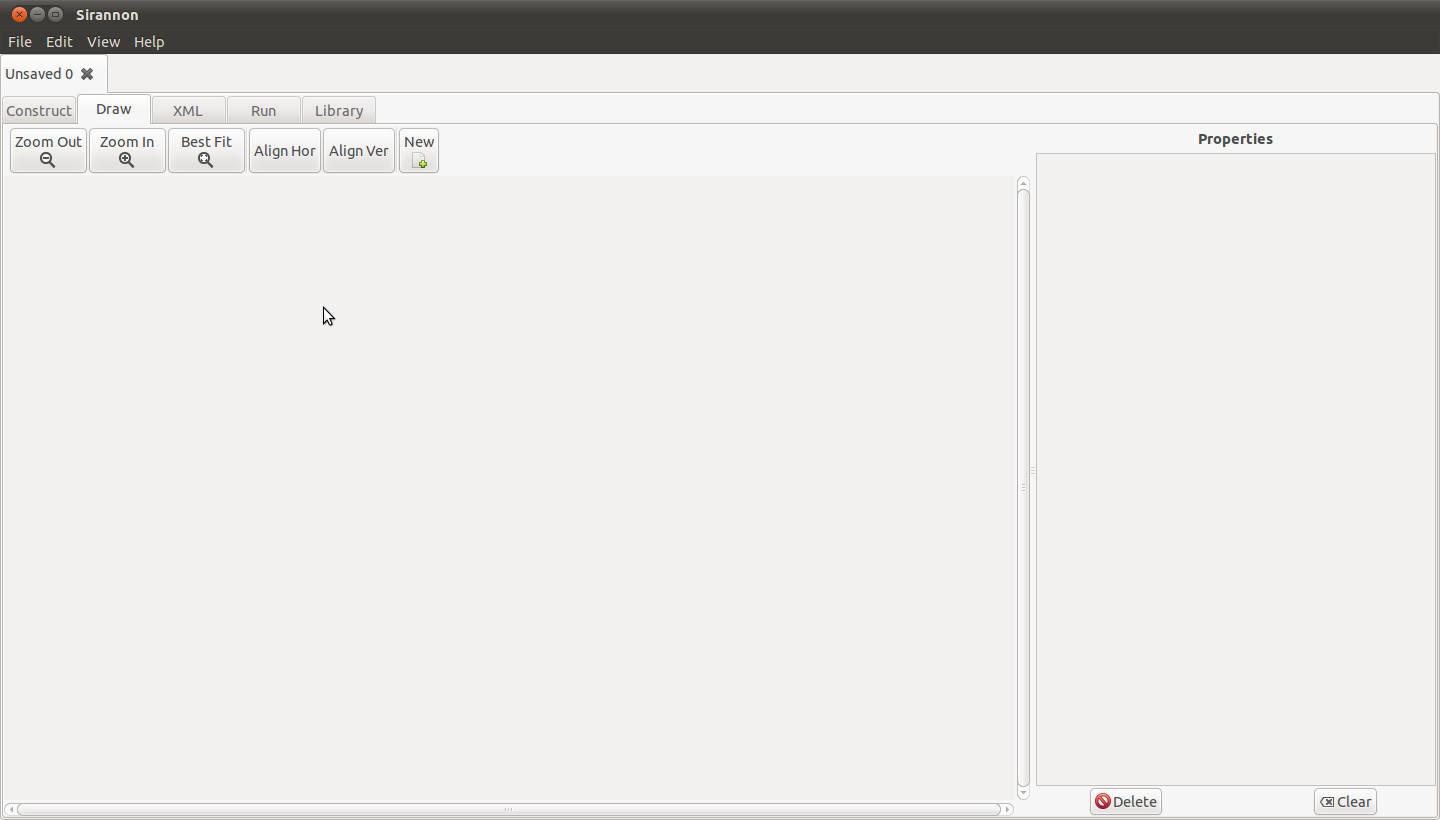
\includegraphics[width=1.0\textwidth]{./images/ui01.png}
	\caption{the user interface}
	\label{fig:6}
\end{center}
\end{figure}
\newpage

\section{Creating your first component}
In order to open the trailer, a reader component is needed. The \textit{ffmpeg-reader} component provides access to the Quicktime container. Let us create this component now. Right-click anywhere in the work area or click on the button 'New' in the toolbar. A menu will appear with the different categories of components. Select \textit{reader}, \textit{ffmpeg-reader}. A new component will appear as seen in \ref{fig:7}. If you left click inside the new component, in the right of the screen an overview of the parameters of the component appears. These parameters are set at sensible defaults, we only need to fill out the \textit{filename} of the trailer. After filling out the \textit{filename}, the result should look as in figure \ref{fig:8}.
\begin{center}
\begin{figure}[!ht]
	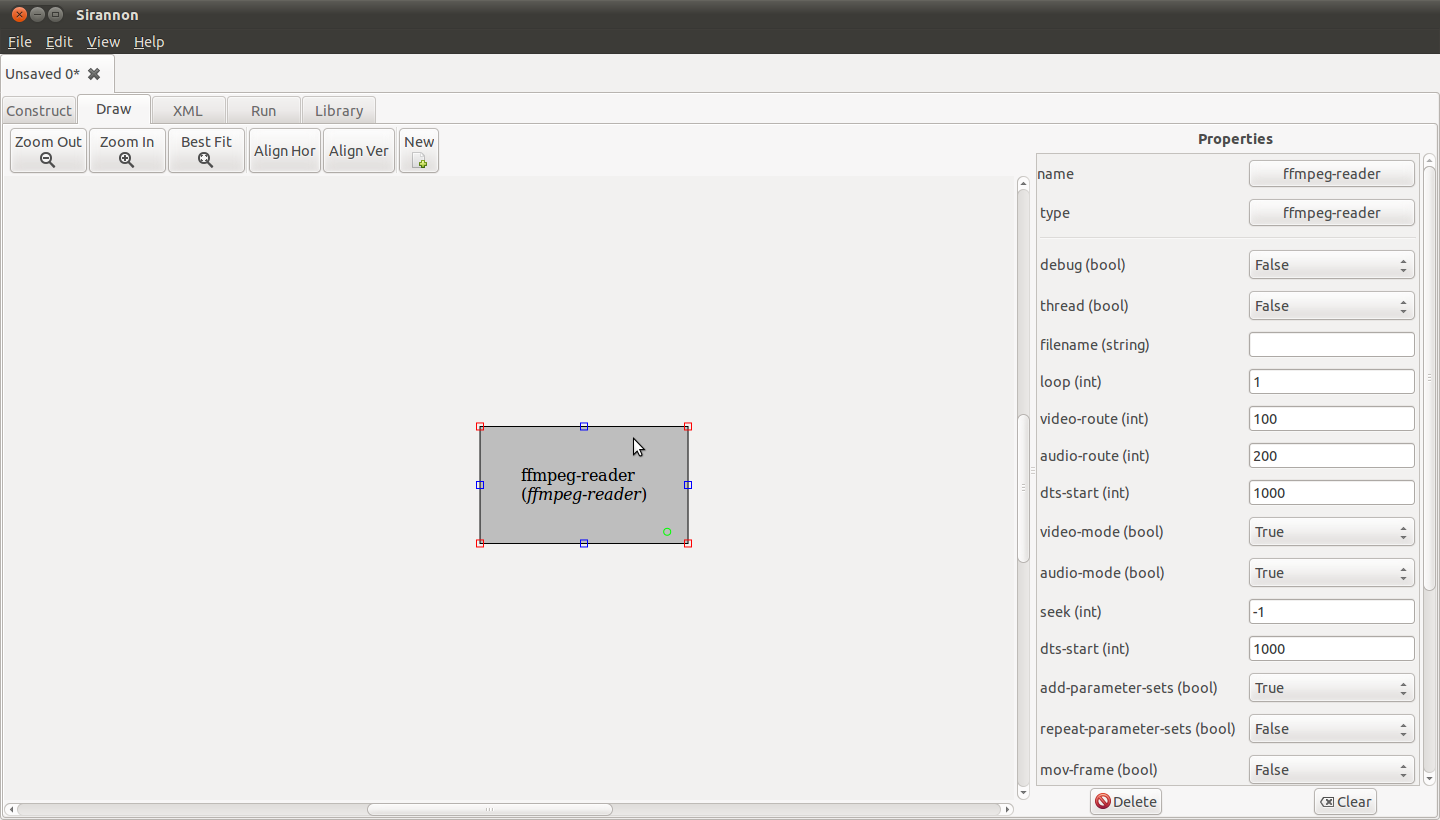
\includegraphics[width=1.0\textwidth]{./images/ui02.png}
	\caption{creating the first component (a)}
	\label{fig:7}
\end{figure}
\end{center}
\newpage
\begin{center}
\begin{figure}[!ht]
	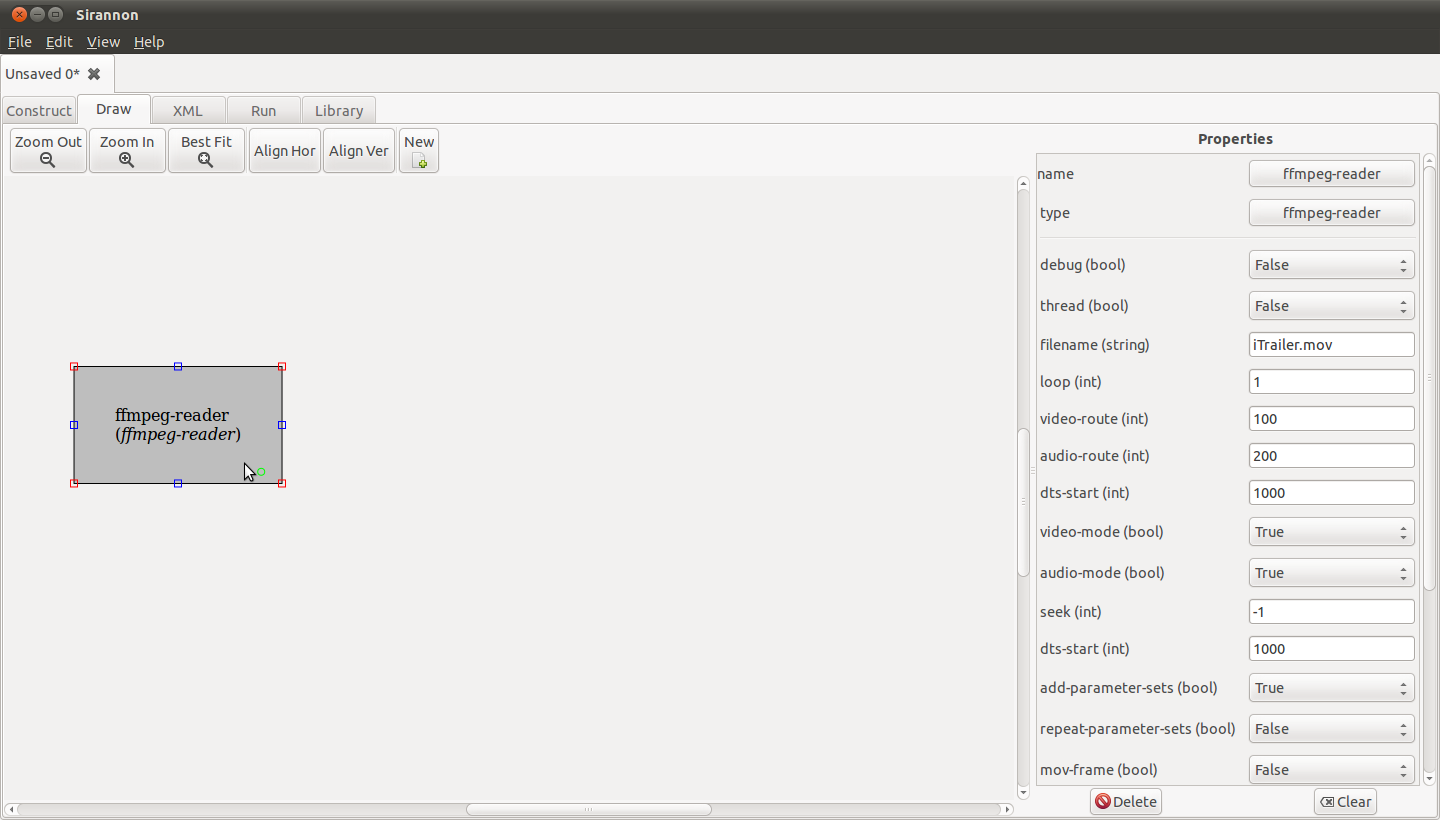
\includegraphics[width=1.0\textwidth]{./images/ui03.png}
	\caption{creating the first component (b)}
	\label{fig:8}
\end{figure}
\end{center}
\newpage

\section{Creating your second component}
The component \textit{ffmpeg-reader} creates packets containing video and audio frames. However, such frames are too large to be sent directly on the network: they have to be packetized into smaller packets. Now let us create the second component. Right-click in the empty work area and select \textit{packetizers}, \textit{PES-packetizer} in the menu. Change the name of the component to \textit{PES-packetizer-video} by clicking on the button next to "name" in the properties area in the right of the screen. Drag this new component to a fitting place, as shown in figure \ref{fig:9}.
\begin{center}
\begin{figure}[!ht]
	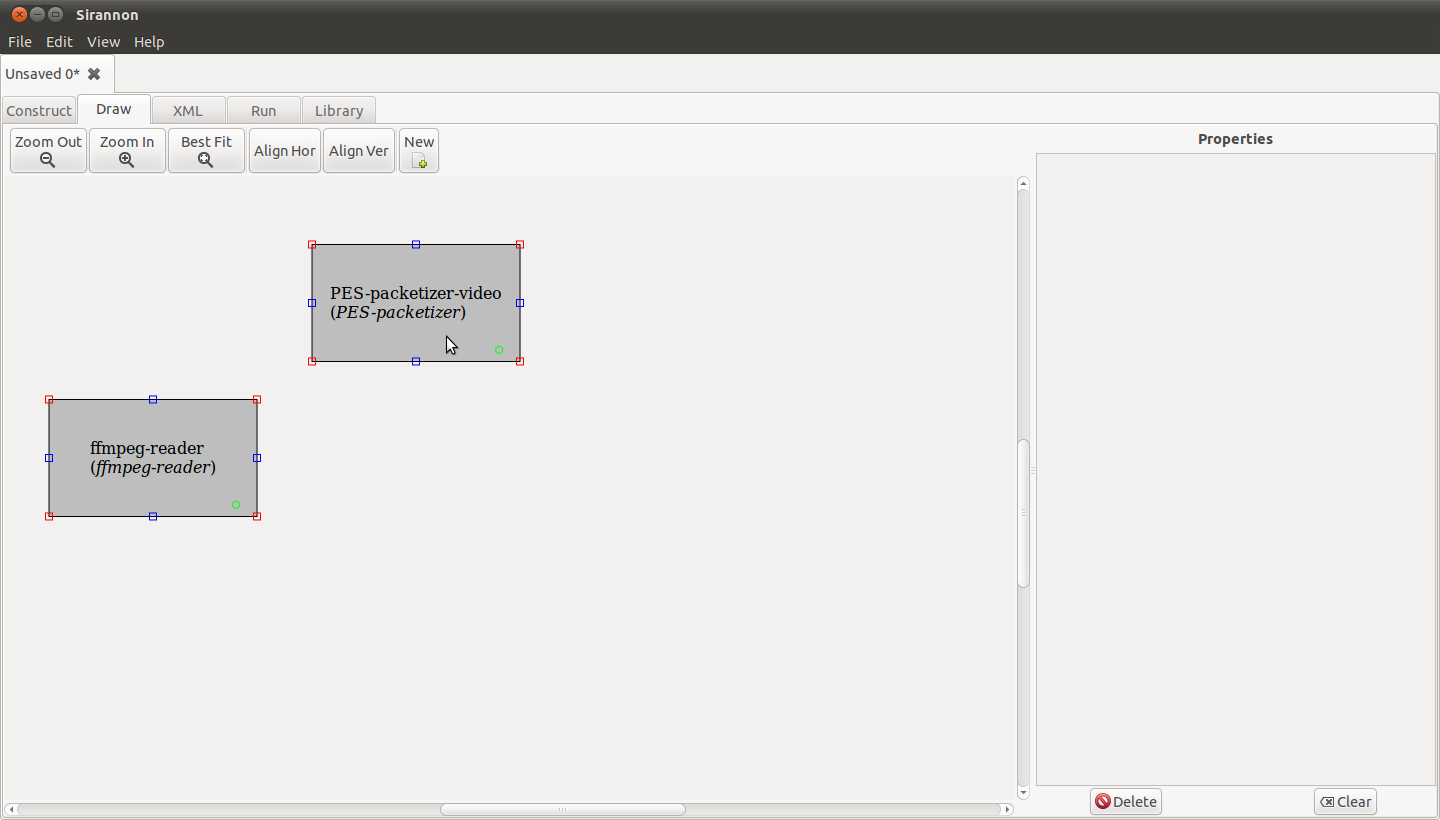
\includegraphics[width=1.0\textwidth]{./images/ui04.png}
	\caption{creating the second component}
	\label{fig:9}
\end{figure}
\end{center}
\newpage

\section{Connecting your components}
The two components need to be connected with each other. When you left-drag from inside one of the blue squares of a component, you will start drawing a line. Left-drag from inside the component \textit{ffmeg-reader} and release the mouse inside one of the blue squares of the component \textit{avc-packetizer}. The connection between the two components is now made and the configuration should now look as in figure \ref{fig:10}.
\begin{center}
\begin{figure}[!ht]
	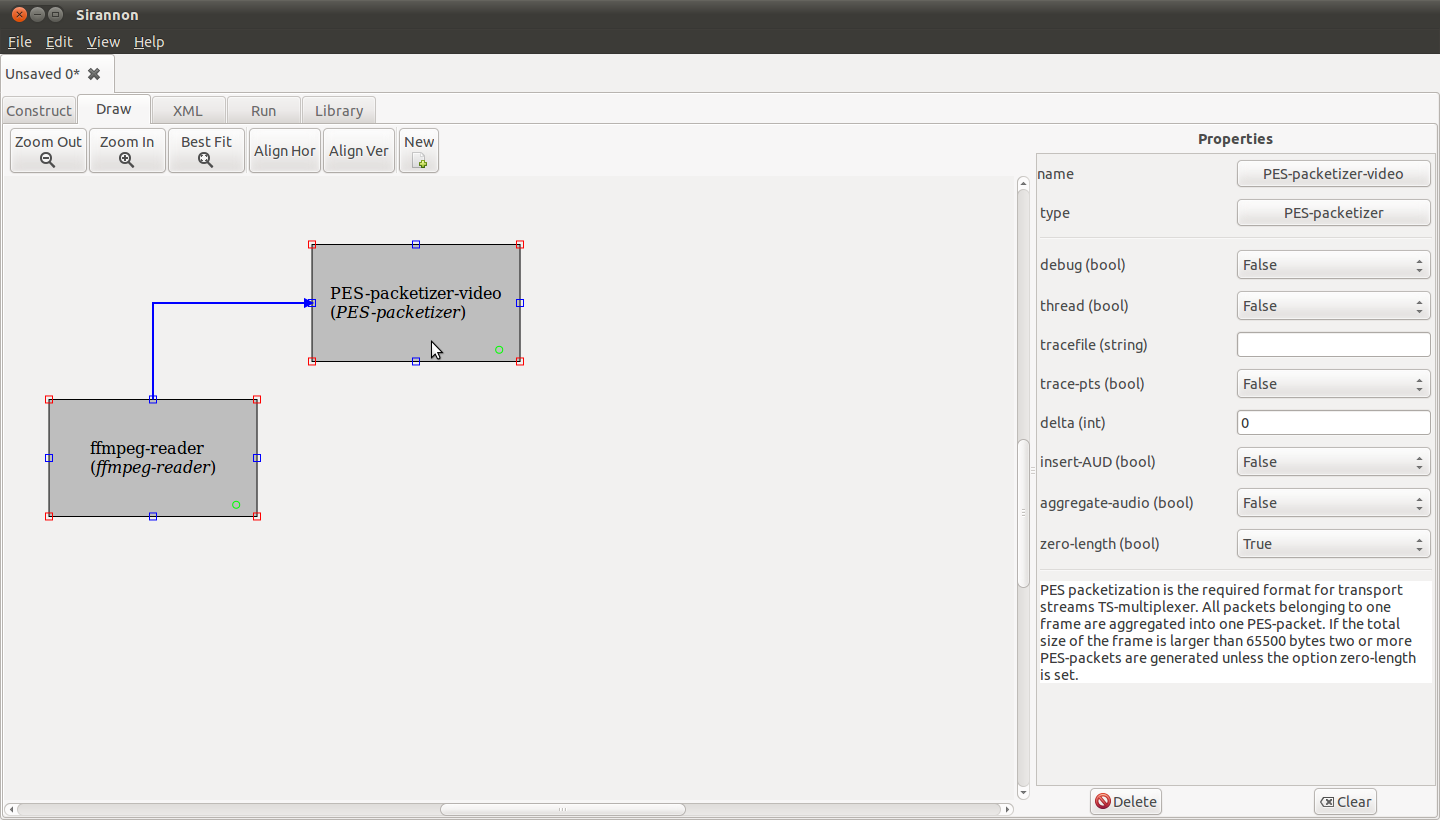
\includegraphics[width=1.0\textwidth]{./images/ui05.png}
	\caption{connecting the two components}
	\label{fig:10}
\end{figure}
\end{center}
\newpage

\section{Creating and connecting your third component}
\label{sec:route}
The \textit{PES-packetizer-video} component will only process video frames. We need a similar packetizer for audio frames. Let us create a third component \textit{PES-packetizer-audio}, found as \textit{packetizer}, \textit{PES-packetizer} in the menu. Change the name of the component to \textit{PES-packetizer-audio}. Connect \textit{ffmpeg-reader} with \textit{PES-packetizer-audio}. No parameters have to be changed for this component either. The result should be as in figure \ref{fig:11}. How can the component \textit{ffmpeg-reader} know on which connection to send packets, since video frames should be sent to \textit{AVC-packetizer} and audio frames to \textit{MP4-packetizer}? In the sirannon each packet is tagged with a number called \textit{xroute}. If you look at the parameters from \textit{ffmpeg-reader}, notice the parameters \textit{video-route} and \textit{audio-route}. Using the default settings, video packets will be tagged with \textit{xroute} $100$ and audio packets with \textit{xroute} $200$. Left click anywhere on connection between \textit{ffmpeg-reader} and \textit{AVC-packetizer}. In the properties area in right of the screen the parameter xroute appears. Since we want to sent only video packets over connection, fill out the value $100$. By default the \textit{xroute} is $0$, meaning all packets are accepted on this connection. If a packet can take multiple paths, for example if multiple connections share the same \textit{xroute} value, a separate copy will be sent over each of those connections. Now left-click on the connection between \textit{ffmpeg-reader} and \textit{MP4-packetizer} and fill out the value $200$, causing audio packets to be sent over this connection.
\begin{center}
\begin{figure}[!ht]
	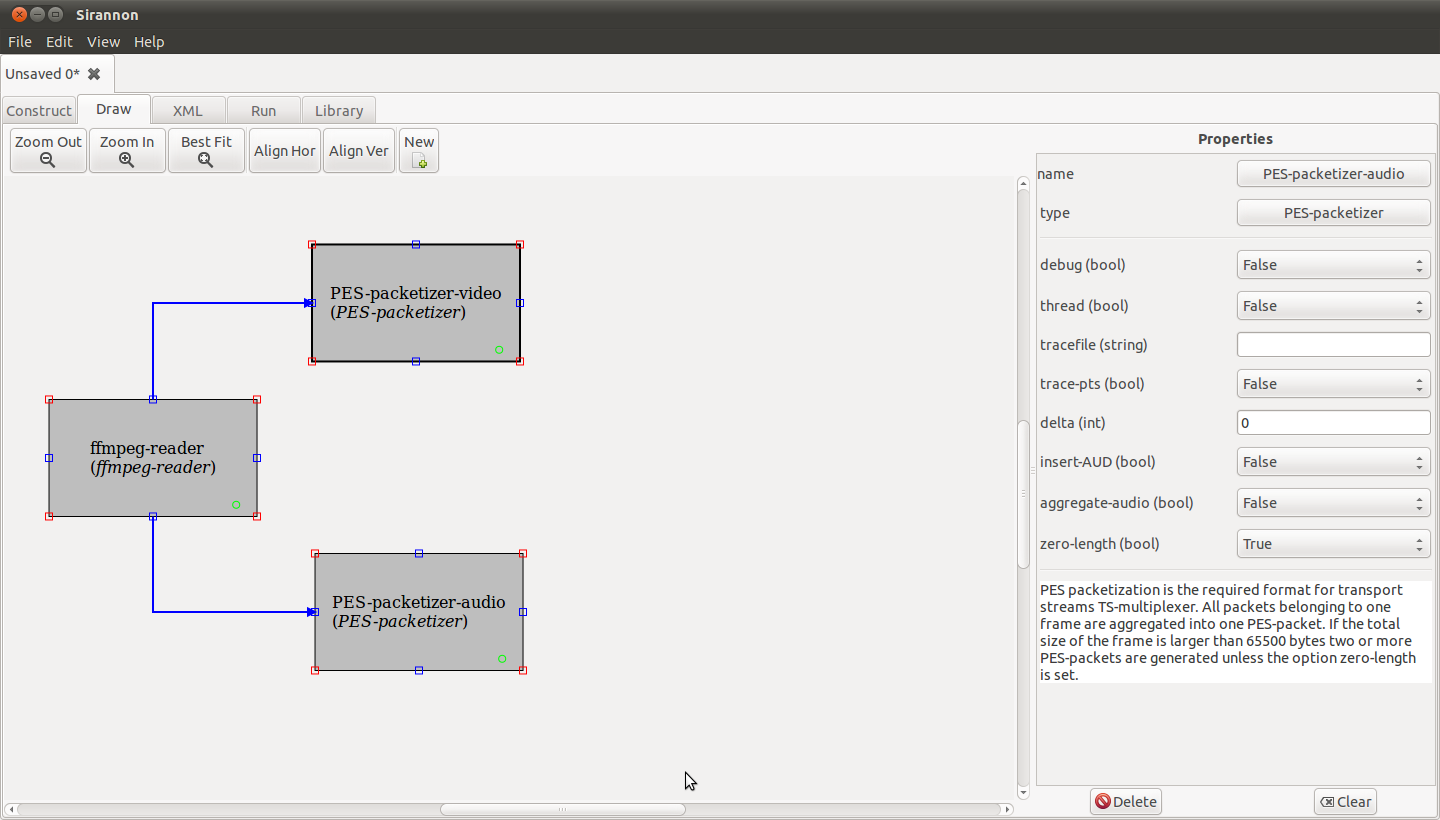
\includegraphics[width=1.0\textwidth]{./images/ui06.png}
	\caption{creating the third component}
	\label{fig:11}
\end{figure}
\end{center}
\newpage

\section{Creating a transport stream}
If we want to send the trailer over a single connection we need to multiplex the trailer into an MPEG2 Transport Stream. Create new component \textit{TS-multiplexer} by selecting \textit{multiplexer}, \textit{TS-multiplexer} from the menu. Connect both packetizers with this new component. The result should look in figure \ref{fig:99}. If you made a mistake, you can always undo using CTRL-Z or selecting undo in the menu.
\begin{center}
\begin{figure}[!ht]
	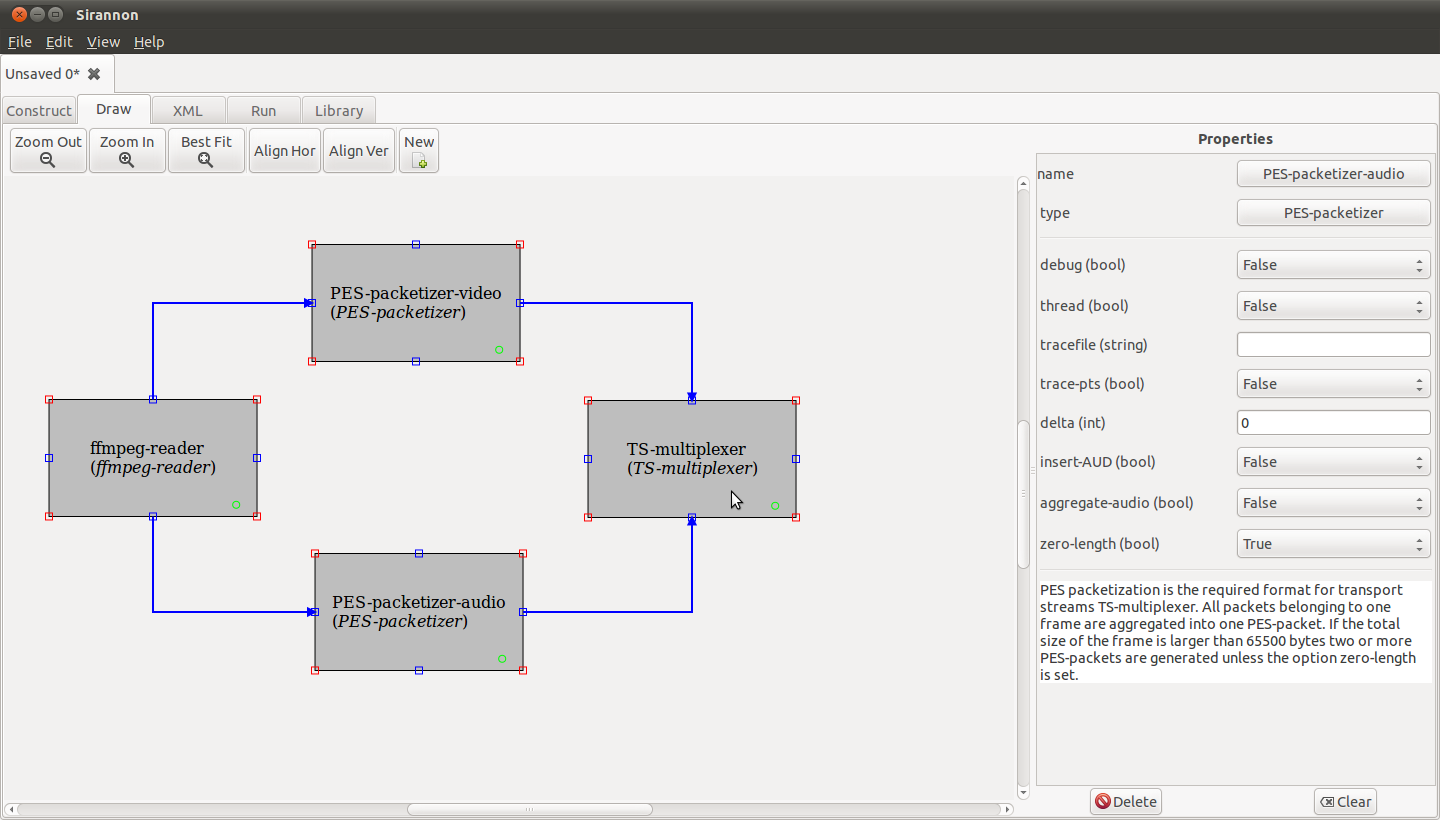
\includegraphics[width=1.0\textwidth]{./images/ui99.png}
	\caption{multiplexing the packets}
	\label{fig:99}
\end{figure}
\end{center}
\newpage

\section{Scheduling the packets}
We need a scheduler to add real-time behavior: it stores packets in a buffer and releases them at the correct time. Create a scheduler by selecting \textit{schedulers}, \textit{frame-scheduler} from the menu. Figure \ref{fig:12} shows the intended result. If your draw area becomes too small you can always zoom out by clicking the appropriate button in the toolbar.
\begin{center}
\begin{figure}[!ht]
	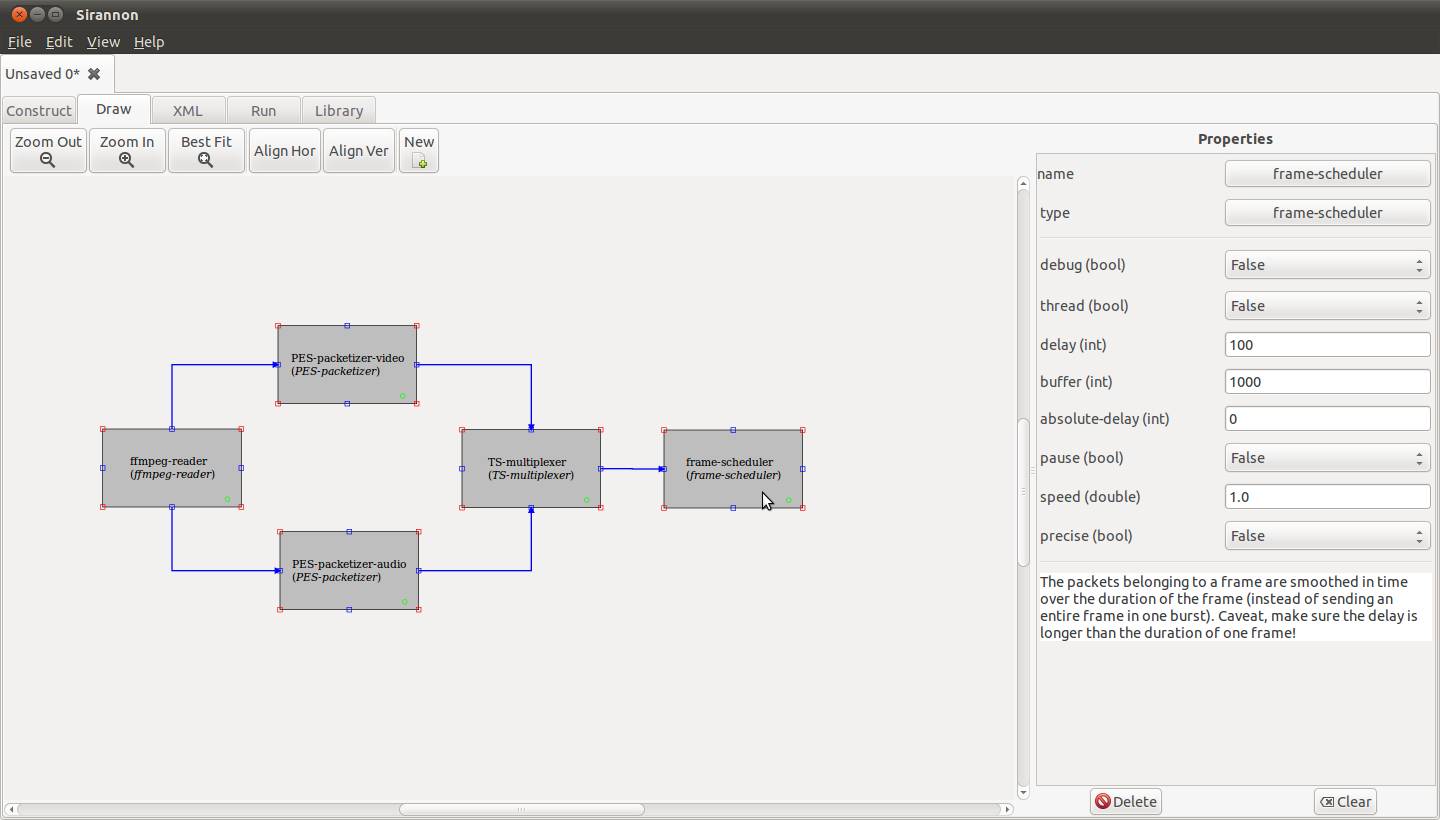
\includegraphics[width=1.0\textwidth]{./images/ui07.png}
	\caption{scheduling the packets}
	\label{fig:12}
\end{figure}
\end{center}
\newpage

\section{Transmitting the packets}
The frames are ready now for transmission: they are packetized in sufficiently small packets, multiplexed into an MPEG2 transport stream and scheduled at the correct time. Let us create an RTP-transmitter. Select \textit{transmitter}, \textit{RTP-transmitter} from the component menu and connect the scheduler with the new transmitter. We have to fill out the source port and destination address. In the properties area for the parameter \textit{port} fill out the value 5000 and for the parameter \textit{client} fill out $127.0.0.1:1234$. Also set the parameter \textit{debug} to \textit{true} for this component. Figure \ref{fig:13} shows the result. 
\begin{center}
\begin{figure}[!ht]
	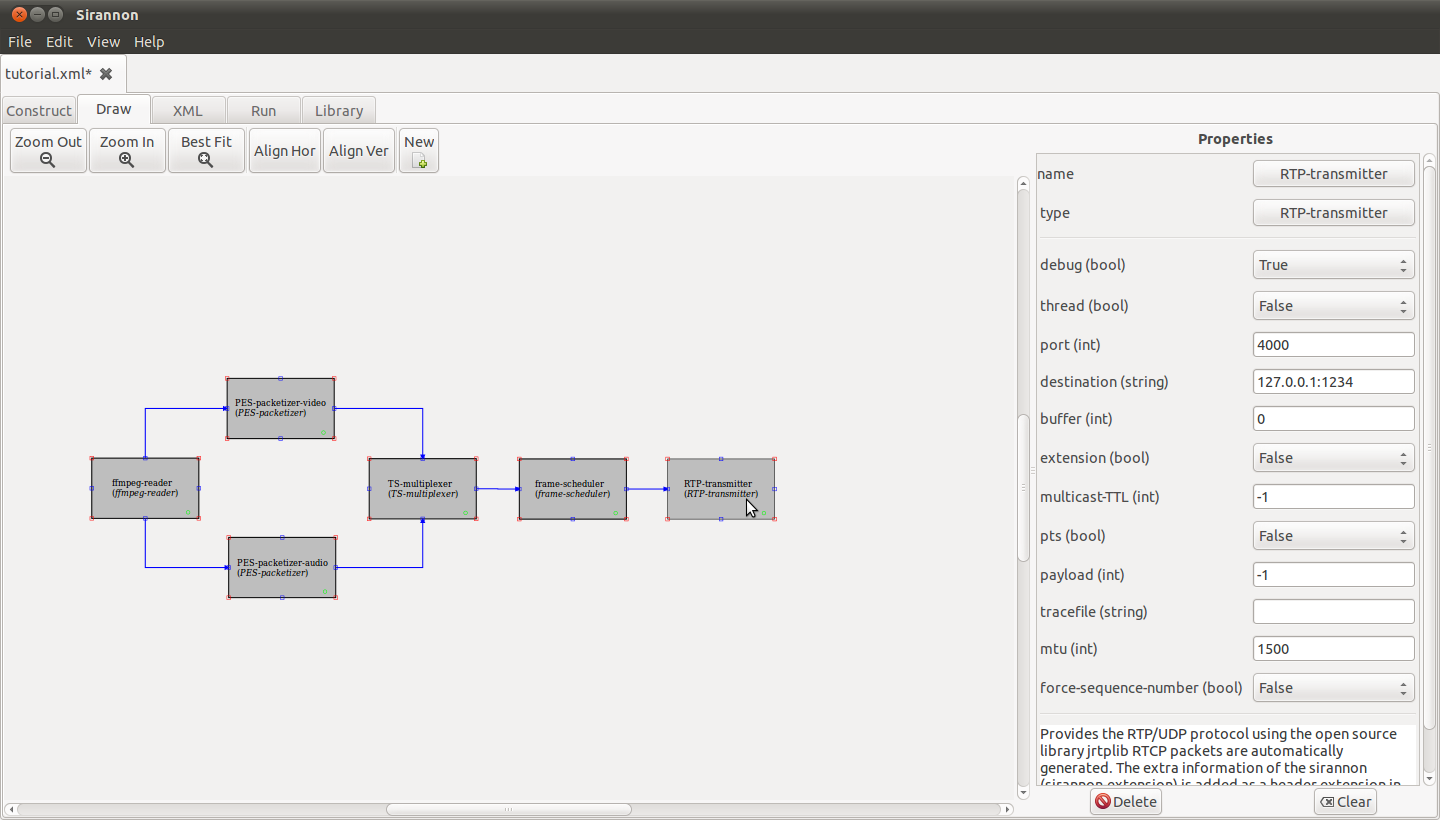
\includegraphics[width=1.0\textwidth]{./images/ui08.png}
	\caption{transmitting the packets}
	\label{fig:13}
\end{figure}
\end{center}
\newpage

\section{Finalizing the chain}
In order to close the sirannon after streaming the sequence, we should place a special block called \textit{sink} at the end of the chain. After the last packet of the sequence has passed through this sink, it terminates the program gracefully. Select \textit{system}, \textit{sink} from the component menu and make a connection form the transmitter to this sink. The result should look as in figure \ref{fig:14}. Zoom out or use best fit if the drawing area is too small.
\begin{center}
\begin{figure}[!ht]
	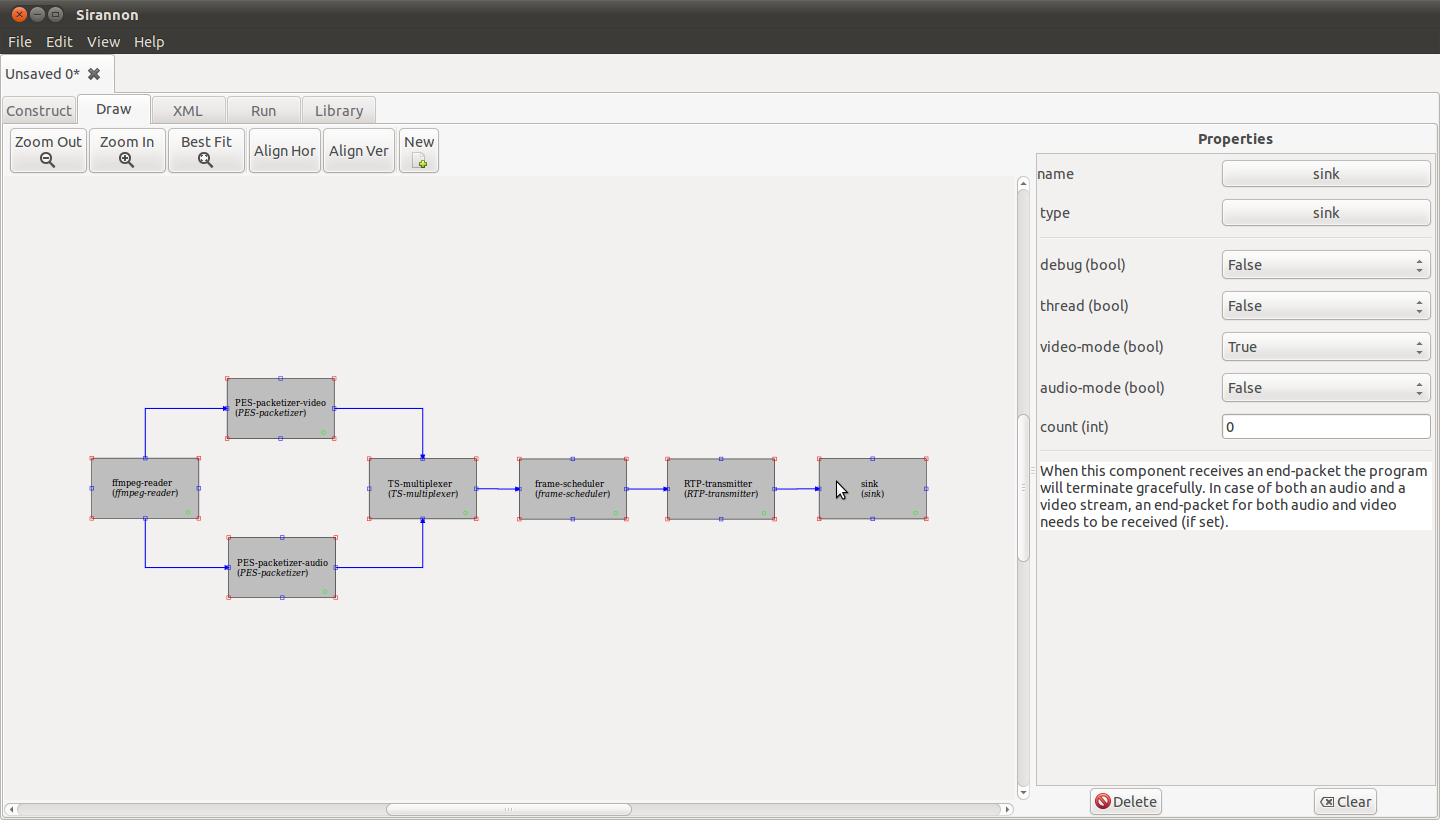
\includegraphics[width=1.0\textwidth]{./images/ui09.png}
	\caption{finalizing the chain}
	\label{fig:14}
\end{figure}
\end{center}
\newpage

\section{Saving and Executing your the configuration}
Now that the configuration is complete, we can save it. In the menu bar under \textit{File} use either \textit{Save} or \textit{Save as} or press \textit{CTRL-S}. We can now run sirannon using the tab "Run". A new tab should appear that looks like in figure \ref{fig:98}.
If the GUI finds the binary it should appear as first item of the command line options. Under Unix you should have compiled and installed the sirannon binary if you wish to continue. If you installed the binary in a different location you can always select that location.

We do not need to fill out the configuration, when you press play the GUI will automatically using the current configuration unless you overwrite it.

\begin{center}
\begin{figure}[!ht]
	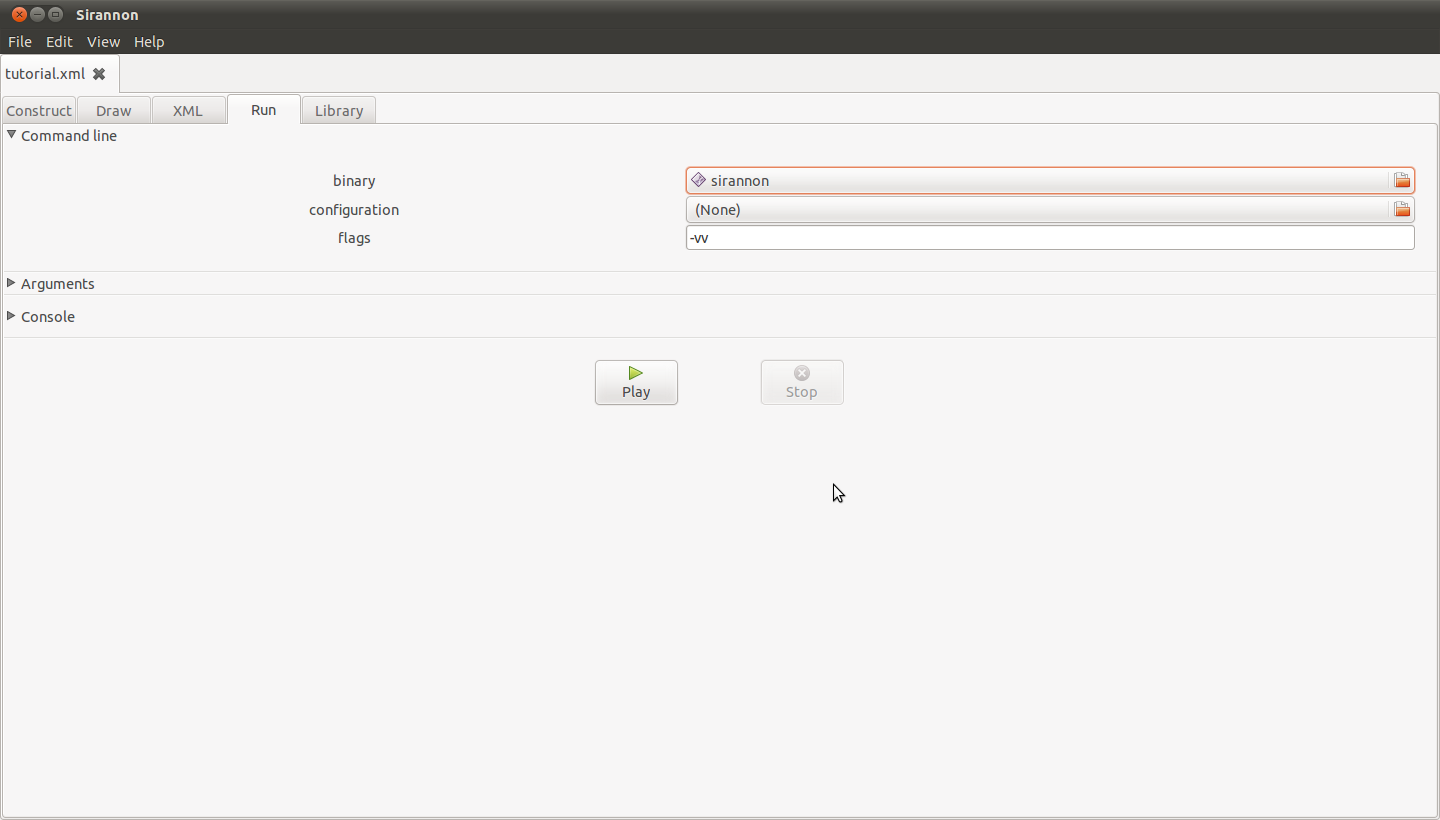
\includegraphics[width=1.0\textwidth]{./images/ui98.png}
	\caption{the "Run" tab}
	\label{fig:98}
\end{figure}
\end{center}
\newpage

Press the large \textit{Play} button. The console window expands and shows the output of the sirannon process. If you filled out an incorrect container for the ffmpeg-reader, sirannon should fail with an error like \texttt{Unhandled RuntimeError: core.ffmpeg-reader: Could not open file(iTrailer.mov)}. If you do not have a sample video at hand you can always download the demo containers from \url{http://sirannon.atlantis.ugent.be/files/demo.tar.bz2}. Bear in mind that for MPEG2 Transport Streams only MPEG video and audio codecs are supported. If you created everything correctly output should appear in the console as in figure \ref{fig:97}.

Once the console is running you can open for example VLC Media Player. Under \textit{Media}, select \textit{Open Network Stream}. Fill out \texttt{rtp://@:1234} as URL. VLC should now start playing the video. \textbf{CAVEAT:} If your sequence uses H.264/AVC, VLC will not have critical information that was transmitted by streamer before VLC launched. You will need to press \textit{Stop} followed by \textit{Play} to fix it. To prevent this behaviour you can set the parameter \textit{repeat-parameter-sets} to \textit{true} for the component \textit{ffmpeg-reader}.

Now the video should be playing as in figure \ref{fig:96}. If it is not working, go over the following check list.
\begin{itemize}
\item Press \textit{Stop} followed by \textit{Play}
\item Is parameter \textit{destination} for \textit{RTP-transmitter} set to \textit{127.0.0.1:1234}?
\item Does the console show an error such as \texttt{Could not open file} or \texttt{Unsupported codec}?
\end{itemize}

\begin{center}
\begin{figure}[!ht]
	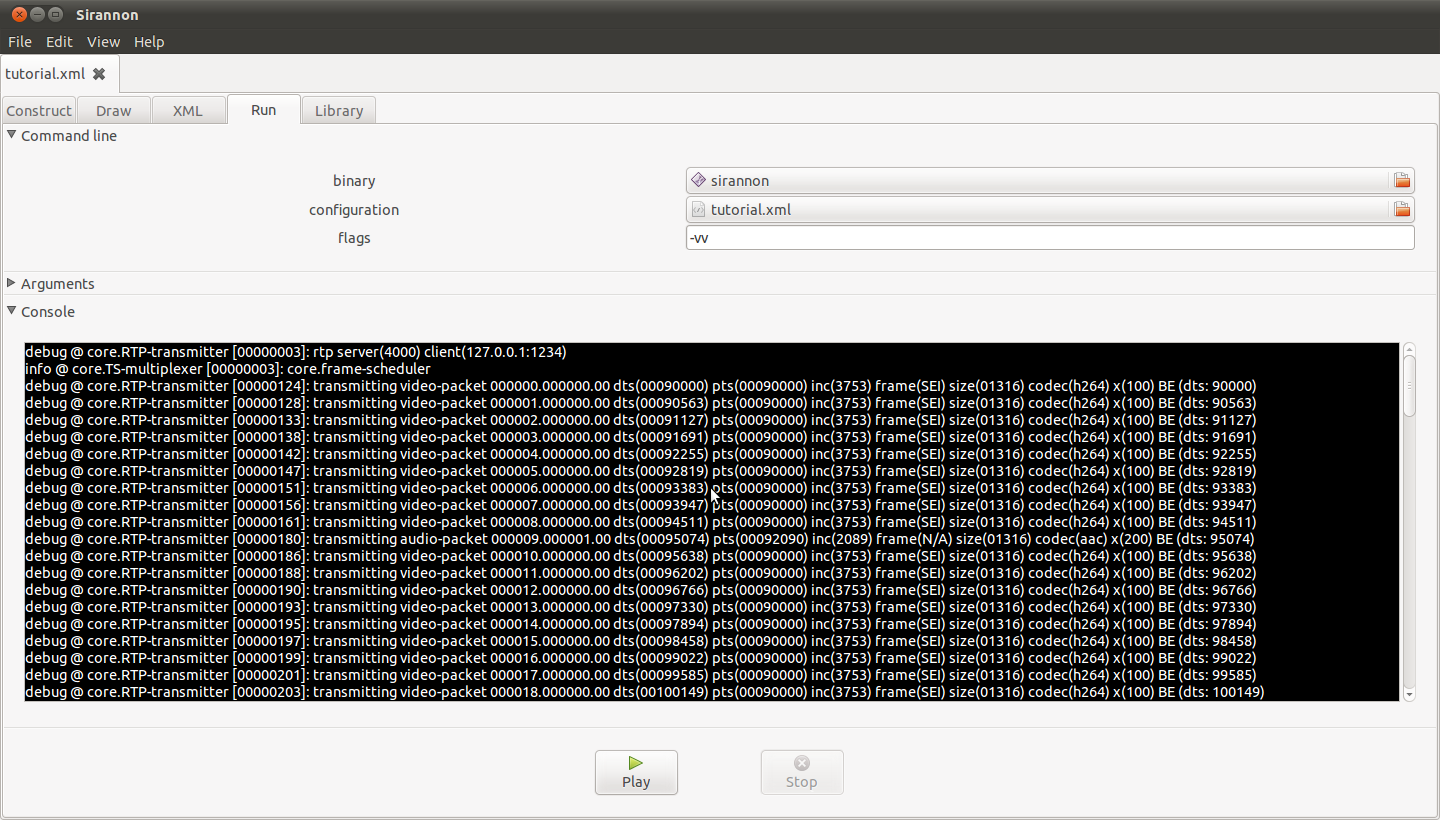
\includegraphics[width=1.0\textwidth]{./images/ui97.png}
	\caption{the console output}
	\label{fig:97}
\end{figure}
\end{center}

\begin{center}
\begin{figure}[!ht]
	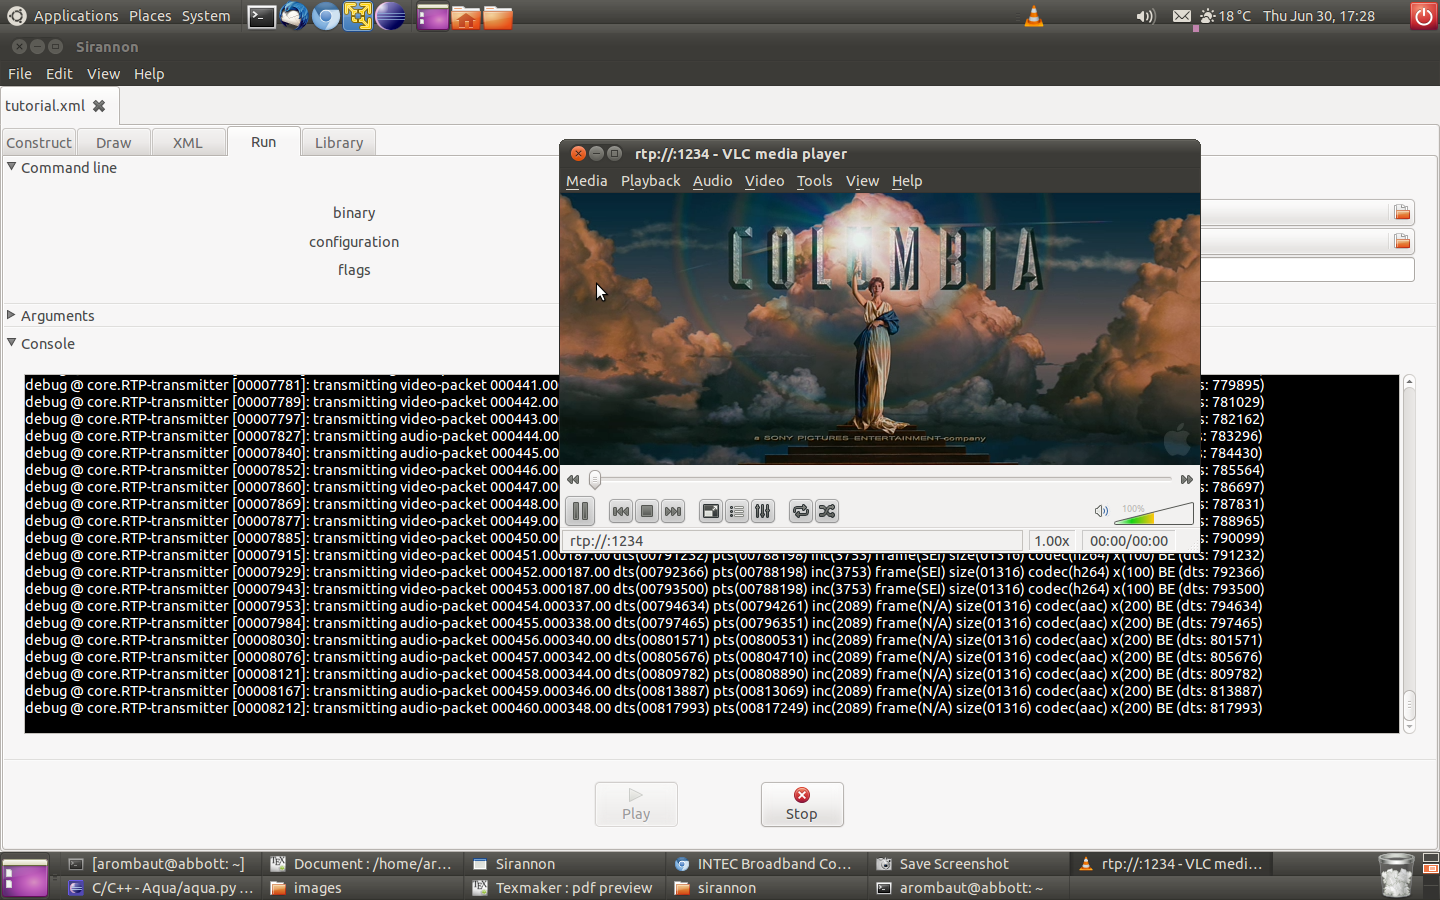
\includegraphics[width=1.0\textwidth]{./images/ui96.png}
	\caption{VLC receiving and playing the stream}
	\label{fig:96}
\end{figure}
\end{center}
\newpage

\chapter{Execution}
\label{chap:exe}
\section{Internal view}
We shortly describe here the internal view of the sirannon in order to understand the parameters in the next section. The basic operation of the sirannon is single threaded. The execution consists of a series of cycles with each cycle aiming to process one frame. The real duration of such a cycle, for example 2ms, is often much lower than the duration of one frame, typically 40ms. The process can sleep during the difference, lowering the CPU load considerably.

\section{Execution parameters} 
Let us introduce three execution parameters. To modify these parameters in the user interface for a configuration, go in the menu bar to \textit{Settings}, \textit{Settings}. These parameters are specific for each configuration.
\begin{enumerate}
\item\textbf{quantum}: in milliseconds, defines the minimum time to process one frame. If processing of a frame took less than this quantum, the process sleeps during the difference, lowering the CPU load. If you match this quantum with the duration of each frame, you get a working performance with minimal CPU load. For example a stream with 25 frames per second or 40 ms per frame, can be streamed using less than 1\% CPU using a quantum of 40ms. If the quantum is set at 0, the process never sleeps, producing very accurate timing (order 1 ms) at the cost of 100\% CPU utilization. default: 0

\item\textbf{simulation}: in microseconds, if this value is greater than 0 the sirannon runs in simulated time. Each cycle the simulated time is increased with this value. This has the advantage of providing arbitrary time precision and possibly faster execution at the cost of losing the real time behavior. For example the simulation of streaming an HD/H264 stream using simulation steps of $40000\mu s$, can be run in $2s$ instead of $40s$ in real time. When \textit{simulation} is defined, the parameter \textit{quantum} is ignored. default: 0

\item\textbf{seed}: if this value is greater than 0, it provides the seed for the random numbers in the sirannon. If the value is 0, the current time is used as seed. default: 0
\end{enumerate}

\section{Command line parameters}
In order to use the configuration files without having to edit them when using differnt content, component parameters (not execution parameters!) can be entered in the form of \$1, \$2, \$3\textellipsis The symbol \$\textit{n} will be replaced by the $n^{th}$ command line parameter after the configuration file (see next section). Use the symbol \$\$ to circumvent this interpretation and represent the character "\$".

\section{Usage}
\begin{verbatim}
sirannon [-cvbh] [-q=NUM[ns|us|ms|s]] [-s=NUM[ns|us|ms|s]] [-r=NUM] FILE [ARG-1] ... [ARG-n]
Run the program with FILE as configuration.

Options:
  -h       Help information
  -b       Build information
  -c       Overview of components
  -v       Verbose, use up to 4 v's to increase the level
  -q=NUM   Quantum in milliseconds
  -s=NUM   Simulation in milliseconds
  -r=NUM   Seed for the random number generator

Arguments:
  ARG-1    Replace any occurrence of "$1" in FILE with ARG-1
  ARG-2    Replace any occurrence of "$2" in FILE with ARG-2
  ARG-NUM  Replace any occurrence of "$NUM" in FILE with ARG-NUM\end{verbatim}

\subsection{Example 1}
\texttt{sirannon -v -q=5 avc-streamer.xml gladiator.avi 127.0.0.1:5000}\newline
In this example we run the configuration file "\textit{avc-streamer.xml}" with two command line parameters: the video file name and destination address. These command line parameters will replace the symbols \$1 and \$2 entered in the configuration file. In addition we set the quantum to 5 ms and print debug messages from toggled components.

\subsection{Example 2}
\texttt{sirannon -b -c}\newline
Prints the build information and the available components. Since no xml file is specified, the program end instantly.


\chapter{Examples}
\label{chap:ex}
The basics of the sirannon were explained in the previous chapters. By using examples, we will demonstrate the many possibilities of the sirannon. In contrast with the tutorial, we will not explain how to construct the configuration in the user interface but we will focus instead on describing the function and structure of different configurations. Sometimes we will refer to specific parameters of components. For a detailed description of the components and a full list of available parameters, refer to the next chapter. The distribution of Sirannon contains for each example the corresponding XML file.

\section{Example 1: a basic streamer}
Let us start with a basic example, even simpler than the tutorial: a basic AVC streamer. Figure \ref{fig:ex:1} shows the schematic. It contains the four basic components: a reader, a packetizer, a scheduler and a transmitter, connected in a chain.
\begin{center}
\begin{figure}[!ht]
	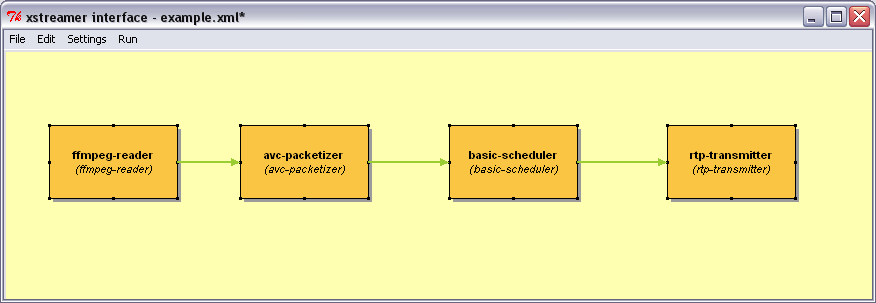
\includegraphics[width=1.0\textwidth]{./images/ex01.png}
	\caption{a basic streamer}
	\label{fig:ex:1}
\end{figure}
\end{center}
\newpage

\section{Example 2: a basic receiver}
The stream sent by the basic streamer can be received by a media player, but the sirannon also can act as a receiver. Hence, the sirannon is more than just a streamer. Figure \ref{fig:ex:3} shows this receiver. The receiver has four components like the basic streamer, performing the reverse operation: a receiver, a scheduler, an unpacketizer and a writer. Received packets are unpacketized into the original frames and those are written back to a file. The scheduler avoid problems such as UDP reordering or duplication. However, the RTP protocol should circumvent these problems, making the scheduler superfluous in this example.
\begin{center}
\begin{figure}[!ht]
	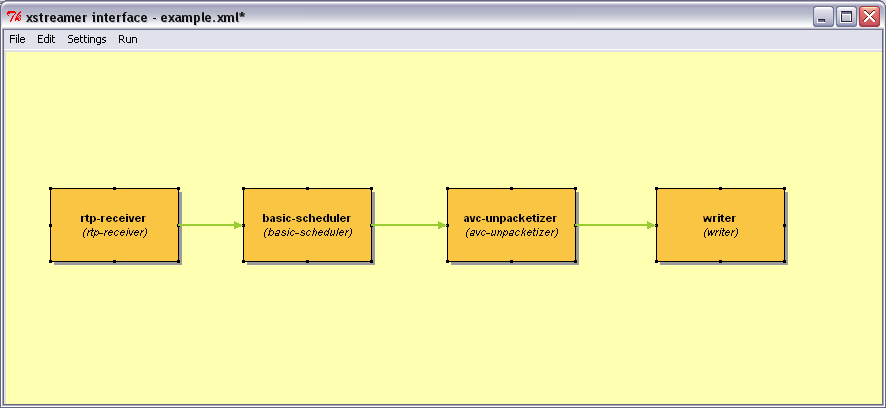
\includegraphics[width=1.0\textwidth]{./images/ex03.png}
	\caption{a basic receiver}
	\label{fig:ex:3}
\end{figure}
\end{center}
\newpage

\section{Example 3: differentiated streaming}
\label{sec:diff}
This example modifies the structure of the basic streamer from example 1 in order to stream over multiple connections. Figure \ref{fig:ex:2} shows the result. Instead of having one \textit{rtp-transmitter}, we now have three. We also add a \textit{frame-classifier} to differentiate the I, P and B frames. The sirannon allows forks in the schematic using a simple routing mechanism based on a label \textit{xroute} per packet. The reader gives each packet an initial \textit{xroute} of 100. A classifier increases the \textit{xroute}\ with a fixed value for each classification. In this example, \textit{frame-classifier} has three parameters I, P and B with values 1, 2 and 3 respectively, producing packets with \textit{xroutes} 101, 102 and 103. The connections between \textit{frame-classifier} and \textit{rtp-transmitter 1, 2 and 3} use \textit{xroutes} 101, 102 and 103 respectively to split the stream. Section \ref{sec:route} also explains this routing system.
\begin{center}
\begin{figure}[!ht]
	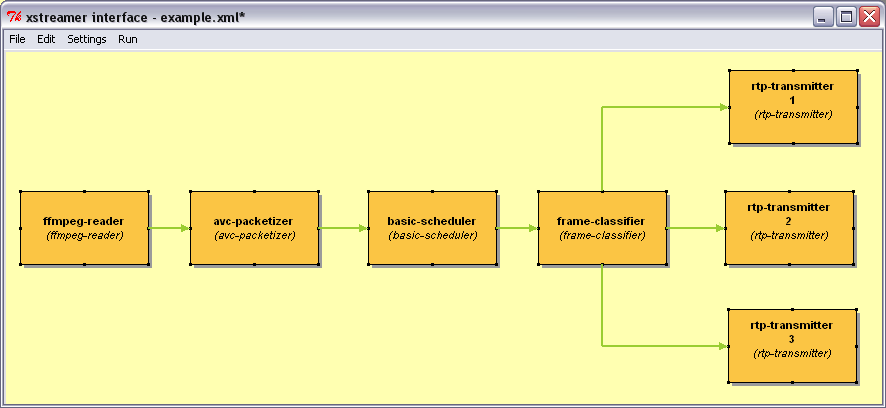
\includegraphics[width=1.0\textwidth]{./images/ex02.png}
	\caption{a differentiated streamer}
	\label{fig:ex:2}
\end{figure}
\end{center}
\newpage

\section{Example 4: proxy}
A differentiated stream cannot be played by standard players such as VLC or Quicktime, because it only accepts one connection for video, not three for example. The sirannon can function as a proxy, converting a differentiated stream into a single stream. Such stream can then be received by standard players. Figure \ref{fig:ex:4} shows the schematic. The function consists of three types of components: three receivers, a scheduler and a transmitter. The packets from the three \textit{rtp-receivers} pass through the scheduler. In this setting, the scheduler is anything but superfluous since the three connections are unsynchronized. The scheduler restores the original order. It uses additional information included by the transmitters in the RTP header extension since the sequence numbers and time stamps from the RTP connections are insufficient to restore the original order. It also gives the merged stream the correct time behavior, so that the \textit{rtp-transmitter} can send the merged stream. This merged stream is then received by a standard player.
\begin{center}
\begin{figure}[!ht]
	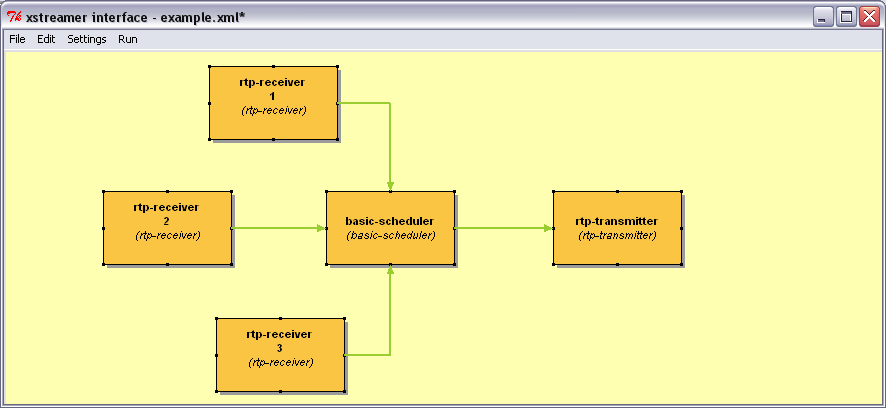
\includegraphics[width=1.0\textwidth]{./images/ex04.png}
	\caption{a proxy}
	\label{fig:ex:4}
\end{figure}
\end{center}
\newpage

\section{Example 5: a packet loss generator}
The sirannon can also run as an offline tool. Figure \ref{fig:ex:5} shows the schematic to introduce packet loss, with a different percentage for each type of frame. The frames are read and packetized by \textit{avc-reader} and \textit{avc-packetizer}. The \textit{frame-classifier} splits the stream into I, P and B packets. For each of these types there is different component \textit{random-classifier 1, 2} or \textit{3} with its specific packet loss. The damage streams are merged and unpacketized by \textit{avc-unpacketizer} and the resulting frames (some of the original frames are lost) are written by the component \textit{writer}.
\begin{center}
\begin{figure}[!ht]
	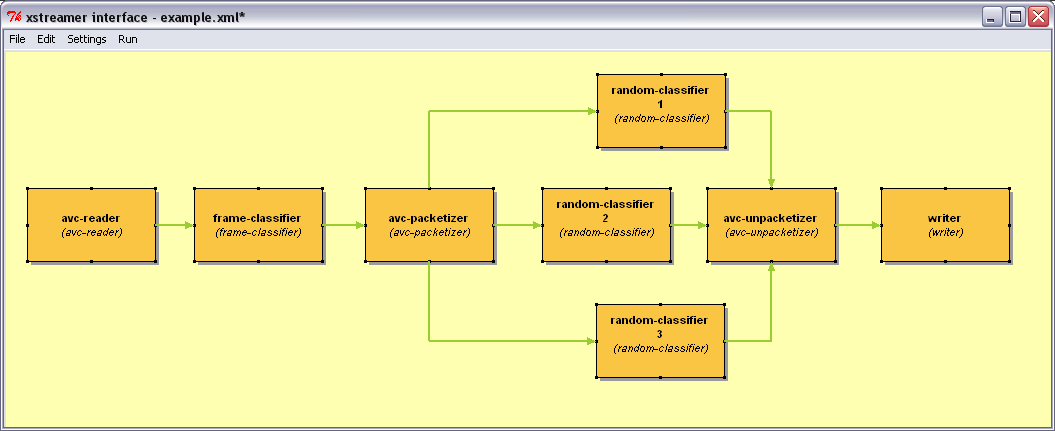
\includegraphics[width=1.0\textwidth]{./images/ex05.png}
	\caption{a packet loss generator}
	\label{fig:ex:5}
\end{figure}
\end{center}
\newpage

\section{Example 6: using transport streams}
The sirannon supports MPEG2 transport streams, widely used in digital television. It multiplexes video, audio and meta-data into one stream that we can send over one connection, as opposed to the default RTP mode where each video, audio or meta-data substream has its own RTP session. Figure \ref{fig:ex:6} shows the configuration. It does not differ that much from the basic streamer. \textit{ffmpeg-reader} opens a Quicktime file containing both video and audio frames and  \textit{xroute} is set at 100 and 200 respectively for video and audio by the reader. Two packetizers create generic PES packets for video and audio respectively. The component \textit{ts-mutliplexer} multiplexes these packets into one transport stream. The two remaining components schedule and transmit the transport stream packets.
\begin{center}
\begin{figure}[!ht]
	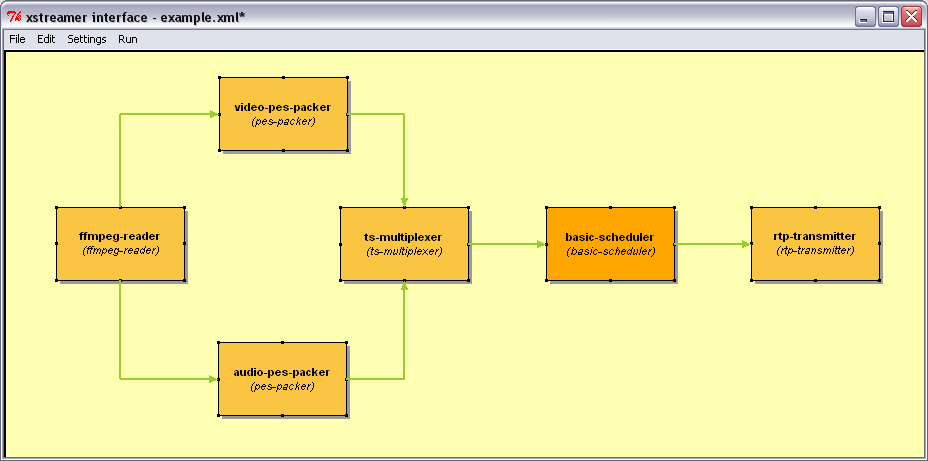
\includegraphics[width=1.0\textwidth]{./images/ex06.png}
	\caption{using transport streams}
	\label{fig:ex:6}
\end{figure}
\end{center}
\newpage

\section{Example 7: using and constructing blocks}
Let us create a simulator to test the behavior of a buffer. Block components allows us to group several component into one component, allowing more readable and parameterized configurations. Figure \ref{fig:ex:7a} shows a \textit{qmatch-buffer} component and three \textit{block} components. Each \textit{block} components uses a configuration file that reads and packetizes a sequence. Figure \ref{fig:ex:7b} shows this configuration. This looks similar to the basic streamer example but it has at the end of the chain an \textit{out} component which sends packets to the surrounding configuration (figure \ref{fig:ex:7a}). In order to obtains precise timing results, we run the sirannon in simulation mode with a simulation step of 1000 $\mu s$.
\begin{center}
\begin{figure}[!ht]
	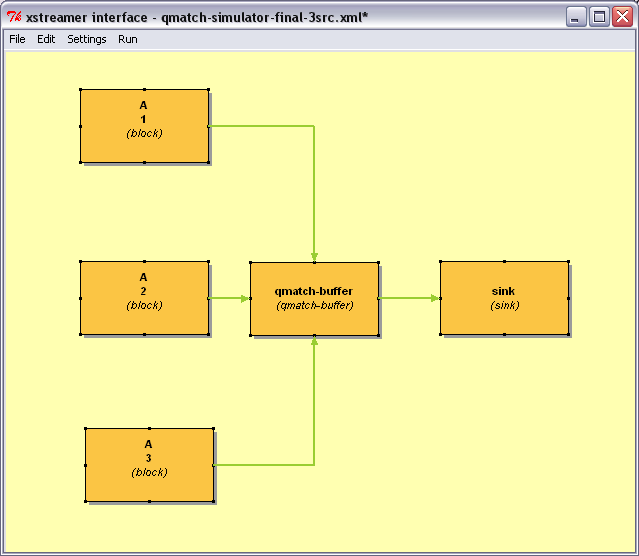
\includegraphics[width=1.0\textwidth]{./images/ex07a.png}
	\caption{simulating a buffer}
	\label{fig:ex:7a}
\end{figure}
\newpage
\begin{figure}[!ht]
	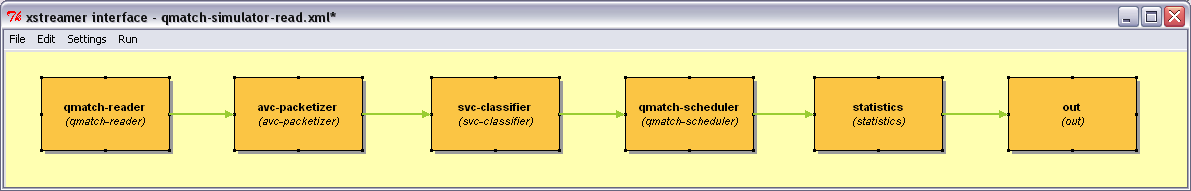
\includegraphics[width=1.0\textwidth]{./images/ex07b.png}
	\caption{streamer contained in the block}
	\label{fig:ex:7b}
\end{figure}
\end{center}
\newpage

\section{Example 8: massive simulation}
Using blocks we can create massive simulators of for example 18 different streams, as shown in figure \ref{fig:ex:8}.
\begin{center}
\begin{figure}[!ht]
	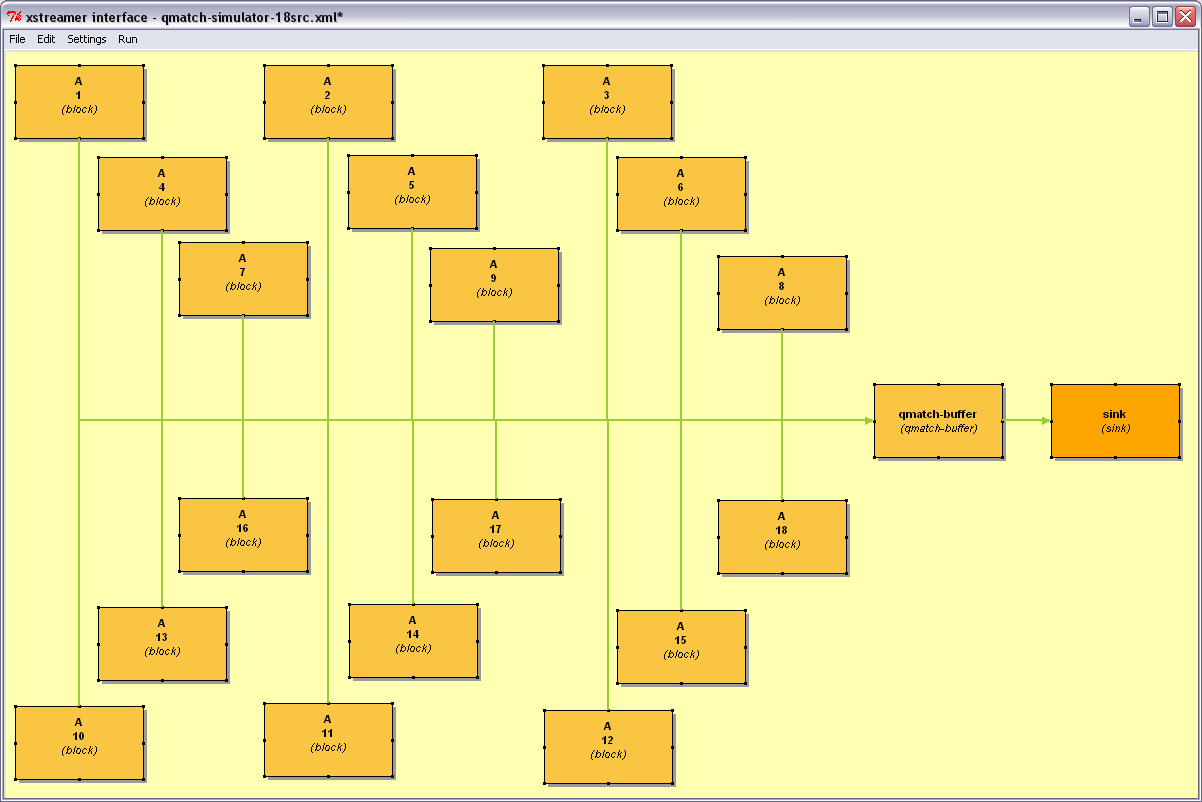
\includegraphics[width=1.0\textwidth]{./images/ex08.png}
	\caption{a massive simulator}
	\label{fig:ex:8}
\end{figure}
\end{center}
\newpage

\chapter{Extending sirannon}
In the source tree \texttt{src/Misc/Example.cpp} describes a good commented example about writing your own component. Place any new sources you create in the folder \texttt{src/Local} and add the flag \texttt{--enable-local} to \texttt{configure}. When adding new sources, rerun \texttt{configure --enable-local}.

\chapter{Components}
\label{chap:components}

Components can have two special parameters:
\begin{itemize}
\item bool \textbf{debug}: if true, the component prints debug information, requires verbose level one or higher (use -v in the command line), default: false
\item bool \textbf{thread}: if true, run the component in a separate thread, default: false 
\end{itemize}
\newpage
\section{classifier}
Classifiers add an offset to the xroute of a packet if it meets a certain condition. See section \ref{sec:diff} for an example. Several classifiers can be chained to obtain a more precision classification.
\begin{itemize}
\item Parameters:
\begin{itemize}
\item bool discard: if true, delete the packet instead if the condition is met, default: false
\item string sender-trace: if defined, the path where to log information about the packets entering the classifier, default: ""
\item string receiver-trace: if defined, the path where to log information about the packets exiting the classifier, implies discard is true, default: ""
\end{itemize}
\end{itemize}
\subsection{avc-classifier}
This components classifies the many different types of NAL units present in H264, far the beyond the common I, B and P frames.
\begin{itemize}
\item Parameters:
\begin{itemize}
\item int I: the offset if the media-packet is an I slice, default: 0
\item int SI: the offset if the media-packet is an SI slice, default: 0
\item int EI: the offset if the media-packet is an EI slice, default: 0
\item int I(B): the offset if the media-packet is an I (data partition B) slice, default: 0
\item int I(C): the offset if the media-packet is an I (data partition C) slice, default: 0
\item int P: the offset if the media-packet is a P slice, default: 0
\item int SP: the offset if the media-packet is an SP slice, default: 0
\item int EP: the offset if the media-packet is an EP slice, default: 0
\item int P(B): the offset if the media-packet is a P (data partition B) slice, default: 0
\item int P(C): the offset if the media-packet is a P (data partition C) slice, default: 0
\item int B: the offset if the media-packet is a B slice, default: 0
\item int EB: the offset if the media-packet is an EB slice, default: 0
\item int B(B): the offset if the media-packet is a B (data partition B) slice, default: 0
\item int B(C): the offset if the media-packet is a B (data partition C) slice, default: 0
\item int E: the offset if the media-packet is a prefix NAL, default: 0
\item int PPS: the offset if the media-packet is a PPS unit, default: 0
\item int SPS: the offset if the media-packet is an SPS unit, default: 0
\item int ESPS: the offset if the media-packet is an extended SPS unit, default: 0
\item int SEI: the offset if the media-packet is a SEI unit, default: 0
\item int default: the offset if the packet does not belong to any of the above, default: 0
\end{itemize}
\end{itemize}
\subsection{count-classifier}
This component classifies or discards every nth frame if 'n % cycle' is non zero. By setting discard to true, this component will essentially discard all but every nth frame.
\begin{itemize}
\item Parameters:
\begin{itemize}
\item int cycle: do not classify every 'cycle * n'th frame, e.g. if cycle is 10, do not classify frames 0, 10, 20, 30, etc., default: 10
\end{itemize}
\end{itemize}
\subsection{fixed-classifier}
Classifies the packets, slice or frames based on fixed indices provided by the user. CAVEAT: Indices must rise strict monotonously; Non slice NAL units such as PPS, SPS, SEI, E, are not counted as slices while different SVC layers are also counted as slices. For example an MVC stream with 4 slices and with 2 layers per frame will be counted as 8 slices.
\begin{itemize}
\item Parameters:
\begin{itemize}
\item string mode: whether the indices inputted in values or values-file specify packets, slices or frames, accepted values: frame, slice, packet, default: frame
\item string values: if defined, a comma seperated string of indices, indicating which packet, slice or frame to classify counted from 0, default: ""
\item string values-file: if defined, a file containing a new line seperated string of indices, indicating which packet, slice or frame to classify counted from 0, default: ""
\item int xroute: offset added to the xroute of the packet if the packet is classified, default: 1
\end{itemize}
\end{itemize}
\subsection{frame-classifier}
Classifies packets based on the type of frame they belong to. The parameter I stands for all sort of I frames (I, IDR, EI, SI...), the same holds for other frame types.
\begin{itemize}
\item Parameters:
\begin{itemize}
\item int I: the offset if the media-packet is an I slice or frame, default: 0
\item int B: the offset if the media-packet is an B slice or frame, default: 0
\item int P: the offset if the media-packet is an P slice or frame, default: 0
\item int default: the offset if the frame type is none of the above, default: 0
\end{itemize}
\end{itemize}
\subsection{gilbert-classifier}
This component has a random chance of classifying a packet using the Gilbert method.
\begin{itemize}
\item Parameters:
\begin{itemize}
\item double alpha: $\in[0,1]$, probability to transit from the GOOD to the BAD state, default: 0.01
\item double beta: $\in[0,1]$, probability to transit from the BAD to the GOOD state, default: 0.1
\item double gamma: $\in[0,1]$, probability to classify a packet in the BAD state, default: 0.75
\item double delta: $\in[0,1]$, probability to classify a packet in the GOOD state, default: 0.01
\item int xroute: offset if the condition is met, default: 1
\end{itemize}
\end{itemize}
\subsection{nalu-drop-classifier}
Drops specific NAL units from an H.264/AVC encoded video stream. The indices of the NAL units to drop are provided in a tracefile. The first NAL unit of the stream has index 1.
\begin{itemize}
\item Parameters:
\begin{itemize}
\item string drop-trace: path to file which contains information on which NAL units to drop. A sample drop-trace file is located in the src/Misc folder., default: ""
\item bool udpmode: set to true in case a UDP receiver is used instead of an RTP receiver. Sequence numbers are retained in UDP mode whereas in case of an RTP receiver and transmitter new sequence numbers are generated., default: false
\end{itemize}
\end{itemize}
\subsection{random-classifier}
This component has a random chance of classifying a packet using a uniform distribution.
\begin{itemize}
\item Parameters:
\begin{itemize}
\item double P(loss): $\in[0,1]$, probability to classify the packet, default: 0.01
\item int xroute: offset if the condition is met, default: 0
\end{itemize}
\end{itemize}
\subsection{svc-classifier}
This component classifies an SVC stream. The partitioning is defined by a series of $(T,D,Q)$ triplets. For each passing NAL unit this series is reverse iterated. If the NAL unit depends on the $n^{th}$ triplet then it is classified as $layer-{n}$. When it didn't depend on any layer it is classified as $layer-{0}$. The triplets are entered in the form of $'T,D,Q:offset'$, for example $'4,0,0:2'$, meaning \textit{'add offset 2 to packets of temporal layer (T) 4 or higher'}.
\begin{itemize}
\item Parameters:
\begin{itemize}
\item int layer: offset for layer 0, default: 0
\item string layer-1: definintion and offset for layer 1, default: ""
\item string layer-2: definintion and offset for layer 2, default: ""
\item string layer-3: definintion and offset for layer 3, default: ""
\item string layer-4: definintion and offset for layer 4, default: ""
\item string layer-5: definintion and offset for layer 5, default: ""
\item string layer-6: definintion and offset for layer 6, default: ""
\item string layer-7: definintion and offset for layer 7, default: ""
\end{itemize}
\end{itemize}
\subsection{time-classifier}
Basic classifier based solely on the real time interval, relative to the first packet. The four time parameters combine to create an interval of the form: $t\in[start,stop[$, when step is defined, it must also hold that: $$t\in\bigcup-{n=1}^{+\infty}[n\cdot step,n\cdot step+delta[$$.
\begin{itemize}
\item Parameters:
\begin{itemize}
\item int start: in ms, the minimum of the range, default: 0
\item int stop: in ms, the maximum of the range, -1 being unlimited, default: -1
\item int step: in ms, the time between two steps, -1 disabling the step effect, default: -1
\item int delta: in ms, the duration of one step, -1 being unlimited, default: -1
\item int xroute: offset if the condition is met, default: 1
\end{itemize}
\end{itemize}
\subsection{timestamp-classifier}
Basic classifier based solely on the decoding time stamp (DTS) interval, relative to the first packet.
\begin{itemize}
\item Parameters:
\begin{itemize}
\item int start: in DTS clock ($90kHz$), the minimum of the interval, default: 0
\item int stop: in DTS clock ($90kHz$), the maximum of the interval, -1 being unlimited, default: -1
\item int xroute: offset if the condition is met, default: 1
\end{itemize}
\end{itemize}
\newpage
\section{core}

\begin{itemize}
\item Parameters:
\begin{itemize}
\item bool debug: if true, print debug info for this component, default: false
\item bool thread: if true, run the component in a seperate thread, default: false
\end{itemize}
\end{itemize}
\newpage
\section{demultiplexer}

\subsection{FFMPEG-demultiplexer}
This component is identical to the component FFMPEG-reader, with the exception that the source is not a file but a stream of chunks from a container.
\begin{itemize}
\item Parameters:
\begin{itemize}
\item string format: container format of the input, default: flv
\item int chunk-size: amount of bytes fed to the FFMPEG IOContext each time, default: 32768
\item int loop: the number of times to play the video, -1 being infinite, 0 interpreted as 1, default: 1
\item int videoroute: the xroute that will be assigned to packets containing video, default: 100
\item int audioroute: the xroute that will be assigned to packets containing audio, default: 200
\item int dts-start: in ms, the timestamp that will be added to the DTS \& PTS of each frame, default: 1000
\item bool video-mode: if true, video will be read from the container, if false video will be ignored, default: true
\item bool audio-mode: if true, audio will be read from the container, if false audio will be ignored, default: true
\item int seek: in ms, the timestamp to jump to into the stream, -1 implying no seek, default: -1
\item int dts-start: in ms, specifies the value of the timestamp of the first frame, default: 1000
\item bool add-parameter-sets: H.264/AVC only, if true, extract the parameter sets from the container and insert them into the stream, default: true
\item bool repeat-parameter-sets: H.264/AVC only, if true, repeat the parameter sets before each IDR frame, default: false
\item bool mov-frame: MOV/MP4/F4V container only, if true, keep frames in the format of the container, as opposed to annex-B H.264/AVC streams with start codes before each NAL unit, default: false
\item bool skip-SEI: if true, remove SEI NALUs from the stream, default: false
\item bool skip-AUD: if true, remove AUD NALUs from the stream, default: false
\end{itemize}
\end{itemize}
\subsection{TS-demultiplexer}
Unmultiplexes an MPEG Transport Stream into the original streams each consisting of series of PES-packets. It performs the reverse operation of ts-multiplexer. The MPEG Transport Stream can be as large as entire multi-channel stream.
\begin{itemize}
\item Parameters:
\begin{itemize}
\item int channel: the selected channel to extract, -1 being all channels, default: -1
\item int video-route: the xroute that will be assigned to packets containing video, default: 100
\item int audio-route: the xroute that will be assigned to packets containing audio, default: 100
\end{itemize}
\end{itemize}
\newpage
\section{high-level}

\subsection{TS-segmenter}
This component ingest a video container and generates a series of transport streams at varies bit rates
\begin{itemize}
\item Parameters:
\begin{itemize}
\item string media: path of the folder in which to search for requested files, default: dat/media
\item string filename: the path of the container to stream (relative to the folder specified by media), default: ""
\item string target: string indicating the target display (iphone, ipad, youtube), default: ""
\item int duration: in seconds the maximum duration of one segment, default: 10
\item int bitrate-0: in kbps, the 1st bit rate set point, if 0, do not transcode and only segment and do not check for more bitrates, default: 0
\item int width-0: the 1st width set point, default: 0
\item int height-0: the 1st height set point, default: 0
\item int bitrate-1: in kbps, the 2nd bit rate set point, if 0, do not transcode and only segment and do not check for more bitrates, default: 0
\item int width-1: the 2nd width set point, default: 0
\item int height-1: the 2nd height set point, default: 0
\item int bitrate-2: in kbps, the 3rd bit rate set point, if 0, do not transcode and only segment and do not check for more bitrates, default: 0
\item int width-2: the 3rd width set point, default: 0
\item int height-2: the 3rd height set point, default: 0
\end{itemize}
\end{itemize}
\subsection{streamer}
This component provides a streaming solution without having to construct a scheme of components. Its many parameters reflect the options of the hidden underlying components (delay, port, destination\textellipsis).
\begin{itemize}
\item Parameters:
\begin{itemize}
\item string filename: the path of the container to stream, default: ""
\item string mode: what content to read from the container (video, audio, default), default: default
\item int loop: the number of times to play the stream, -1 being infinite, 0 interpreted as 1, default: 1
\item int seek: the time index to seek to into the container, default: 0
\item bool aggregate: option of some packetizers, default: false
\item int multiplexer-delay: delay of the multiplexer, used for transport streams or RTMP, default: 0
\item string scheduler: which sort of scheduler to use (basic, frame, gop, window), default: basic
\item int scheduler-buffer: in ms, the buffer size in time of the scheduler, default: 1000
\item int scheduler-delay: in ms, the delay of the scheduler, default: 0
\item double loss: if larger than 0, randomly lose packets with the give chance, default: 0.0
\item string transmitter: type of the transmitter(rtp, udp, tcp), default: rtp
\item int port: source port of the transmitter, default: 4000
\item string destination: destination of the transmitter, default: 127.0.0.1:5000
\item bool ts-mode: if true, multiplex the streams into a transport stream, default: false
\item bool RTMP-mode: if true, muliplex the streams into RTMP chunk streams as output from this component, default: false
\item int RTMP-streamID: streamID used for each RTMP chunk stream, default: 1
\item int RTMP-video-chunkID: RTMP chunk stream ID for video, default: 7
\item int RTMP-audio-chunkID: RTMP chunk stream ID for audio, default: 6
\item int RTMP-chunk-size: chunk size for the RTMP chunk streams, default: 4096
\end{itemize}
\end{itemize}
\newpage
\section{media-client}
Media Clients connect to servers and retrieve a stream using a particular protocol. The component outputs frames just as would a a Reader component. In this way streams can be requested and captured (using for example \textit{FFMPEG-writer} or \textit{writer}) or resent using a different protocol (for example converting an RTMP stream to a HTTP stream). Proxy applications for Media Servers (RTMP-proxy, RTMPT-proxy, RTSP-proxy, HTTP-proxy) use this feature.
\begin{itemize}
\item Parameters:
\begin{itemize}
\item string url: the url to retrieve, default: ""
\item bool auto-play: if true, instantly play the stream, default: true
\end{itemize}
\end{itemize}
\subsection{HTTP-capture}
Requests and receives a stream via HTTP. Keeps the container and generates chunks from it.
\begin{itemize}
\item Parameters:
\begin{itemize}
\item int chunk-size: in bytes, the size of the chunks from the container to generate, default: 65536
\end{itemize}
\end{itemize}
\subsection{HTTP-client}
Requests and receives a stream via HTTP. Demultiplexes the container and generates frames.
\begin{itemize}
\item Parameters:
\begin{itemize}
\item string format: the format of the container, if not defined, guess the format based on the extension in the URL, default: ""
\item bool M3U: if true, the URL links to an extended M3U file used by Apple Live HTTP Streaming. The URLs contained in the M3U response will be contacted in turn., default: false
\end{itemize}
\end{itemize}
\subsection{RTMP-client}
Requests and receives a stream via RTMP. Generates audio and video frames.
\begin{itemize}
\item Parameters:
\begin{itemize}
\item bool mov-frame: if true, keep the frames in MOV/MP4 structure for AVC and AAC, default: false
\item int chunk-size: in bytes, the size of the chunks from the container to generate, default: 65536
\end{itemize}
\end{itemize}
\subsection{RTMPT-client}
Requests and receives a stream via RTMPT. Generates audio and video frames.
\begin{itemize}
\item Parameters:
\begin{itemize}
\item int polling: in ms, the time interval between two successive HTTP POSTs during play, default: 1000
\end{itemize}
\end{itemize}
\subsection{RTSP-client}
Requests and receives a stream via RTSP. Generates audio and video frames.
\newpage
\section{media-server}
Media Servers are complex components, listening to a specific TCP port for incoming connections and dynamically creating a session as nested component for each new connection. URLs in the request should be of the form: \texttt{<protocol>://<server-address>/<application>/<media>}. For example \texttt{rtmpt://myserver.com/FILE/flash/example.flv} with server(\texttt{myserver.com}), application(\texttt{FILE}), media(\texttt{flash/example.flv}). Each session creates a nested component of the type \textit{application} given in the URL. Typical applications are FILE, HTTP, RTMP-proxy, RTMPT-proxy, RTSP-proxy, HTTP-proxy.
\begin{itemize}
\item Parameters:
\begin{itemize}
\item string interface: if defined, listen to incoming connections on this specific interface, default: ""
\item string media: path of the folder in which to search for requested files, default: dat/media
\end{itemize}
\end{itemize}
\subsection{HTTP-server}
Listens for incoming HTTP connections. Does not support pausing or seeking. In the URL use application HTTP for file based transfer of requested file. Use the application FILE@FORMAT (eg. FILE@FLV, FILE@WEBM) to change the container type. Example URLs: \texttt{http://myserver.com/HTTP/demo.mov}, \texttt{http://192.168.1.3/FILE@FLV/demo.mov}
\begin{itemize}
\item Parameters:
\begin{itemize}
\item int port: listen to this port for incoming connections, default: 80
\item bool cache: if true, cache generated HLS segments, default: false
\item bool cached: if true, used cached segments and playlists when available, default: false
\item int segment: in seconds, the duration of one HLS segment, default: 10
\item int high: in kbit/s, the bitrate of the high quality HLS encoding, default: 1000
\item int medium: in kbit/s, the bit rate of the medium quality HLS encoding, default: 500
\item int low: in kbits/s, the bit rate of low quality HLS encoding, default: 200
\end{itemize}
\end{itemize}
\subsection{RTMP-server}
Listens for incoming RTMP connections. Supports pausing and seeking. Performs a cryptographical handshake to enable Flash Player to play H.264/AVC and MPEG4-Audio.
\begin{itemize}
\item Parameters:
\begin{itemize}
\item int port: listen to this port for incoming connections, default: 1935
\end{itemize}
\end{itemize}
\subsection{RTMPT-server}
Listens for incoming RTMPT connections. This is the tunneled version of RTMP.
\begin{itemize}
\item Parameters:
\begin{itemize}
\item int port: listen to this port for incoming connections, default: 80
\end{itemize}
\end{itemize}
\subsection{RTSP-server}
Listens for RTSP connections. Supports pausing, but not seeking.
\begin{itemize}
\item Parameters:
\begin{itemize}
\item int port: listen to this port for incoming connections, default: 554
\end{itemize}
\end{itemize}
\newpage
\section{miscellaneous}

\subsection{GOP-splitter}
Cyclically classifies each GOP by increasing the original xroute, so that xroute cycles through [route,route+split[
\begin{itemize}
\item Parameters:
\begin{itemize}
\item int split: in how many parts to split the stream, default: 1
\item bool sync: if true, drop all frames until the first PPS/SPS/IDR packet, default: false
\end{itemize}
\end{itemize}
\subsection{PCAP-writer}
Captures packets using a filter and saves those to a file. Uses libpcap for capturing. Needs to have permission to access the interfaces (eg. sudo).
\newline Availability: Unix\begin{itemize}
\item Parameters:
\begin{itemize}
\item string interface: the name of device on which to capture, default: eth0
\item string filename: the path of the file where to write the captured packets, default: ""
\item string filter: if defined, overwrite the built-in filter, default: ""
\item int port: the UDP port on which to listen for traffic (when using the built-in filter), default: 1234
\item int bitrate: in Mbps, estimated bitrate of stream which determines the underlying buffer size. When unsure of the bitrate, use a royal upper limit. If the debug reports dropped packets, increase this value., default: 20
\end{itemize}
\end{itemize}
\subsection{YUV-display}
Creates a rudimentary video player with no user controls save 'ESC' (which forcibly terminates the video). This component displays immediately any YUV frame it receives. Sirannon must be compiled with the option --with-libSDL to use this component.
\newline WARNING: this component is in a beta version and might not function properly.\begin{itemize}
\item Parameters:
\begin{itemize}
\item int width: in pixels, if defined, the width of the video display, otherwise obtain the information from the MediaPackets containing the YUV frames (pPckt->desc->width), default: -1
\item int height: in pixels, if defined, the width of the video display, otherwise obtain the information from the MediaPackets containing the YUV frames (pPckt->desc->height), default: -1
\item bool full-screen: if true, display the video full screen, default: false
\end{itemize}
\end{itemize}
\subsection{example}
Example component demonstrating the basic API of a functional component
\begin{itemize}
\item Parameters:
\begin{itemize}
\item int test: input variable, default: 5
\item bool foo: an example flag, default: false
\end{itemize}
\end{itemize}
\subsection{fake-reader}
Generates random YUV frames with specified dimensions and/or targetted bitrate.
\begin{itemize}
\item Parameters:
\begin{itemize}
\item int width: the width of the fake frame, default: 1920
\item int height: the height of the fake frame, default: 1080
\item int bits-per-pixel: the number of bits per pixel of the fake frame, default: 12
\item double fps: the number of frames per second, default: 25.
\item int bitrate: if defined, overwrite the bitrate implied by the combination of fps and frame dimensions, default: -1
\item int duration: in ms, if defined the duration of the sequence, otherwise generate frames indefinately, default: -1
\item int mtu: if > 0, divide each frame into packets of maximum mtu size, default: -1
\end{itemize}
\end{itemize}
\subsection{frame-analyzer}
This component parses elementary MPEG-1, MPEG-2, MPEG-4 or H.264/AVC streams to determine the frame type.
\subsection{gigabit-transmitter}

\begin{itemize}
\item Parameters:
\begin{itemize}
\item string destination: the destination, default: 10.10.0.1:1234
\item int port: the source port, default: 4000
\item int mtu: the size of each generated packet (including headers), default: 1450
\item int bitrate: in megabits per seconds, bitrate of the generated stream, default: 100
\item int fps: number of frames per second, default: 25
\end{itemize}
\end{itemize}
\subsection{live-reader}
This component finds a component a runtime and creates a route from that component to this. It also buffers the received packets untill the component is scheduled. Using this technique a live captured stream can be tapped into and routed to this component.
\begin{itemize}
\item Parameters:
\begin{itemize}
\item string url: if defined, create a route from the component out which uses this url, default: ""
\end{itemize}
\end{itemize}
\subsection{restamp}
This components buffers as many packets as the reordering delay and release them we correctly generated DTSs inferred from PTS only streams. This component is only useful when the DTS is corrupted or undefined. CAVEAT: Two packets with the same PTS will cause a RuntuimeError.
\begin{itemize}
\item Parameters:
\begin{itemize}
\item int delay: the maximal reordering delay in packets, default: 2
\end{itemize}
\end{itemize}
\subsection{statistics}
This component generates at regular intervals information about the passing stream
\begin{itemize}
\item Parameters:
\begin{itemize}
\item int interval: in ms, the amount of time between two reports, -1 disables the reports, default: 5000
\item string log: if defined, the path where to log information about the passing packets, default: ""
\item string label: if defined, label used for each entry in the log, this is needed when sending multiple statistics output to one single file, default: ""
\item bool append: if true, append data to the log, if false, overwrite the log, default: true
\item int overhead: the amount of header overhead from network headers to add to the packet size, default: 0
\item bool draw: if true, when an end-packet is received, draw a graph of the bandwidth, requires that \textit{log} is defined, default: false
\end{itemize}
\end{itemize}
\subsection{svc-analyzer}
This component constructs an inter layer bandwidth comparison at the end of a passing svc stream. A 3D graph is constructed with for each layer a cube scaled with the relative weight of the layer in the total bandwidth. The graph is generated as a maple worksheet (\url{www.maplesoft.com}).
\begin{itemize}
\item Parameters:
\begin{itemize}
\item string filename: the path of the maple worksheet with extension .mws, default: ""
\item int dimension: in how many dimensions to scale the cube (1, 2 or 3), default: 1
\end{itemize}
\end{itemize}
\subsection{time-splitter}
Cyclically classifies each time interval by increasing the original xroute, so that xroute cycles through [route,route+split[
\begin{itemize}
\item Parameters:
\begin{itemize}
\item int split: in how many parts to split the stream, default: 1
\item int interval: in ms, the duration of one part, default: 10000
\item bool key: if true, split only if the frame is a keyframe, if false, omit this condition, default: false
\end{itemize}
\end{itemize}
\newpage
\section{multiplexer}
Multiplexers buffer MediaPackets coming from different sources and multiplex those based on the DTS of each MediaPacket. Unmultiplexers perform the reverse operation and restore the original streams.
\begin{itemize}
\item Parameters:
\begin{itemize}
\item int delay: in ms, the minimal amount of data present for each stream of the multiplex before the next packet is released, default: 1000
\item int streams: the number of different streams required before multiplexing, -1 omits this requirement, default: -1
\end{itemize}
\end{itemize}
\subsection{FFMPEG-multiplexer}
Joins packets from different source into a container (no file!) supported by FFMPEG (eg. FLV, WEBM, MP4). The container is released in a stream of MediaPackets containing chunks of the container.
\begin{itemize}
\item Parameters:
\begin{itemize}
\item int chunk-size: in bytes, the maximum size of each chunk, default: 262144
\item string format: format of the container given as file extension (eg. flv, webm, mov, mp4, avi), default: flv
\item bool streamed: if true, disables seeking backwards into the generated chunks, default: false
\end{itemize}
\end{itemize}
\subsection{TS-multiplexer}
Multiplexes audio and video into an MPEG Transport Stream (TS). CAVEAT: If the video or audio come from different readers, you must set the parameter streams or initial-delay, or the component will throw an error.
\begin{itemize}
\item Parameters:
\begin{itemize}
\item int mtu: in bytes, the maximum size of an aggregated packet, typically for an iMTU of 1500 it means 7 Transport Stream packets (1370 bytes), default: 1500
\item bool aggregate: if true, several transport stream packets will be aggregated until their size would exceed the iMTU, default: true
\item int shape: in ms, the amount of media to multiplex each pass, this value overwrites the value of delay, default: 200
\item int pcr-delay: in ms, how much the PCR is in advance of the DTS, the pcr-delay must be lower than the initial DTS of the reader component, default: 400
\item int mux-rate: in kbps, if -1, no fixed multiplexing rate, if 0, the component will guess the mux rate based on the bitrate of the input, if > 0, use this value as mux-rate, default: -1
\item bool continuous-timestamps: if true, use the PCR clock as timestamp for the transport stream, if false, use the timestamps of the PCR stream as timestamps for the transport stream, default: true
\item bool interleave: if false, all transport stream packets belonging to one frame from a PID are consecutive, if true, they are interleaved with transport stream packets from other PIDs (e.g. audio), default: true
\item bool psi-on-key: if true, generate an extra PSI triplet (SDT, PAT and PMT) before the start of every key frame of the PCR stream, default: false
\end{itemize}
\end{itemize}
\subsection{std-multiplexer}
Joins packets from different sources by only ensuring that the DTS and other timing information rise monotonely. This is a requirement for many protocols and containers.
\subsection{unit-multiplexer}
Joins packets from different sources by only ensuring that the unitnumber rises monotonely.
\newpage
\section{packetizer}

\begin{itemize}
\item Parameters:
\begin{itemize}
\item string tracefile: if defined, the path of trace where to log information about the split packets, default: ""
\item bool trace-pts: if true, write the PTS instead of the DTS in the log file, default: false
\end{itemize}
\end{itemize}
\subsection{AC3-packetizer}
Packetizes AC3 audio frames into packets suitable for RTP as defined in (draft) RFC 4184.
\begin{itemize}
\item Parameters:
\begin{itemize}
\item int mtu: in bytes, the maximum size of a network packet, default: 1500
\item bool draft: if true, fill out the header according to the draft version of RFC 4184; this is the version supported by live555/vlc/mplayer, default: true
\end{itemize}
\end{itemize}
\subsection{AMR-packetizer}
AMR and AMR-WB packets are aggregated into packets of (near) MTU size according to RFC 3267
\newline WARNING: this component is in a beta version and might not function properly.\begin{itemize}
\item Parameters:
\begin{itemize}
\item int mtu: in bytes, the maximum size of a network packet, default: 1500
\item int maxptime: in milliseconds, if >= 0, the maximum duration of an aggregate frame, if < 0, omit this requirement, default: 200
\end{itemize}
\end{itemize}
\subsection{AVC-packetizer}
Packetizes H264 frames into packets suitable for the network as defined in RFC 3984.
\begin{itemize}
\item Parameters:
\begin{itemize}
\item int iMTU: in bytes, the maximum size of a network packet, default: 1500
\item bool aggregate: if true, aggregate small packets into one network packet, default: false
\end{itemize}
\end{itemize}
\subsection{MP2-packetizer}
Packetizes MPEG1\&2 audio and video frames into packets suitable for the network as defined in RFC 2250.
\begin{itemize}
\item Parameters:
\begin{itemize}
\item int mtu: in bytes, the maximum size of a network packet, default: 1500
\end{itemize}
\end{itemize}
\subsection{MP4-packetizer}
Packetizes MPEG4 audio and video frames into packets suitable for the network as defined in RFC 3640.
\begin{itemize}
\item Parameters:
\begin{itemize}
\item int mtu: in bytes, the maximum size of a network packet, default: 1500
\item bool aggregate: if true, aggregate small packets into one network packet, default: false
\end{itemize}
\end{itemize}
\subsection{PES-packetizer}
PES packetization is the required format for transport streams TS-multiplexer. All packets belonging to one frame are aggregated into one PES-packet. If the total size of the frame is larger than 65500 bytes two or more PES-packets are generated unless the option zero-length is set.
\begin{itemize}
\item Parameters:
\begin{itemize}
\item int delta: in ms, the amount of time to add to DTS/PTS to make sure is substractable by a PCR, default: 0
\item bool insert-AUD: if true, add AUDs before each H.264 frame, default: false
\item int audio-per-PES: number of audio frames per PES-packet, default: 1
\item bool zero-length: video only, if true, set 0 as PES-packet-length and generate a single PES-packet per frame, default: true
\end{itemize}
\end{itemize}
\subsection{RTMP-packetizer}
This packetizer produces an RTMP chunk stream from the ingested MediaPackets. Such a stream can directly be sent to a Flash Media Server. Unpacketization of this stream is done by the component RMTP-client internally.
\begin{itemize}
\item Parameters:
\begin{itemize}
\item int chunk-ID: the identifier for this RTMP chunk stream, default: 5
\item int stream-ID: the identifier to which global stream this RTMP chunk stream belongs, default: 1
\item int chunk-size: in bytes, the maximum size of each RTMP chunk, default: 128
\end{itemize}
\end{itemize}
\subsection{default-packetizer}
For each new stream creates at runtime a fitting packetizer depending on the codec or the parameter type.
\begin{itemize}
\item Parameters:
\begin{itemize}
\item string type: if defined, force every packetizer to be of this type, useful for forcing PES-packetizer for example, default: ""
\end{itemize}
\end{itemize}
\subsection{sirannon-packetizer}
This simple and generic packetizer can handle any content. However, this packetization is internal to Sirannon and is not recognized by other players. Use sirannon-unpacketizer to unpacketize this stream again.
\begin{itemize}
\item Parameters:
\begin{itemize}
\item int mtu: in bytes, the maximum size of a network packet, default: 1500
\end{itemize}
\end{itemize}
\newpage
\section{reader}
Readers form the primary source of data in the sirannon. When the file reaches its end, a reader either closes the file, generating an end-packet or loops creating a reset-packet. A reader checks if no buffers downstream (typically a scheduler buffer) are full before processing the next frame.
\begin{itemize}
\item Parameters:
\begin{itemize}
\item string filename: the path of the file to open, default: ""
\item int loop: the number of times to play the video, -1 being infinite, 0 interpreted as 1, default: 1
\item int video-route: the xroute that will be assigned to packets containing video, default: 100
\item int audio-route: the xroute that will be assigned to packets containing audio, default: 200
\item int dts-start: in ms, the timestamp that will be added to the DTS \& PTS of each frame, default: 1000
\end{itemize}
\end{itemize}
\subsection{avc-reader}
Reads in a raw H264 video file. Each generated \textit{MediaPacket} contains one H.264 NAL-unit, possibly generating multiple \textit{MediaPackets} per frame.
\begin{itemize}
\item Parameters:
\begin{itemize}
\item bool skip-SEI: if true, ignore the SEI NAL-units, default: false
\item bool skip-AUD: if true, ignore the AUD NAL-units, default: false
\item bool mov-frame: if true, convert NAL-units into MP4/MOV/F4V frames, default: false
\end{itemize}
\end{itemize}
\subsection{basic-reader}
Reads in any container in large chunks. Its main use is the HTTP transmission in chunks of a container.
\begin{itemize}
\item Parameters:
\begin{itemize}
\item int chunk-size: in bytes, the maximum size of a chunk, default: 64000
\item int length: in ms, if > 0, provides the reader with the duration of the file so it can guess the DTS, default: 0
\end{itemize}
\end{itemize}
\subsection{ffmpeg-reader}
Reads in a wide variety of containers supported by ffmpeg. Audio and video are put into different MediaPackets. Per cycle, the reader processes one video frame (if present) and associated audio, possibly generating multiple packets. A separate end- or reset-packet is generated for audio \& video. Note, ffmpeg-reader can also process audio only files.
\begin{itemize}
\item Parameters:
\begin{itemize}
\item bool video-mode: if true, video will be read from the container, if false video will be ignored, default: true
\item bool audio-mode: if true, audio will be read from the container, if false audio will be ignored, default: true
\item int min-ts: in ms, the timestamp to jump to into the stream, -1 implying no seek, default: -1
\item int max-ts: in ms, the maximum timestamp to read from the file, -1 implying no limit, default: -1
\item int dts-start: in ms, specifies the value of the timestamp of the first frame, default: 1000
\item bool add-parameter-sets: H.264/AVC only, if true, extract the parameter sets from the container and insert them into the stream, default: true
\item bool repeat-parameter-sets: H.264/AVC only, if true, repeat the parameter sets before each IDR frame, default: false
\item bool mov-frame: MOV/MP4/F4V container only, if true, keep frames in the format of the container, as opposed to annex-B H.264/AVC streams with start codes before each NAL unit, default: false
\item bool skip-SEI: if true, remove SEI NALUs from the stream, default: false
\item bool skip-AUD: if true, remove AUD NALUs from the stream, default: false
\item bool fix-PTS: if true, parse H.264 frames to extract the POC from which to calculate the correct PTS, default: false
\end{itemize}
\end{itemize}
\newpage
\section{receiver}
Receivers provide the interface from the network for the following protocols: UDP, TCP and RTP/UDP.
\begin{itemize}
\item Parameters:
\begin{itemize}
\item int port: reception port, default: 5000
\item int video-route: the xroute that will be assigned to packets containing video, default: 100
\item int audio-route: the xroute that will be assigned to packets containing audio, default: 200
\item int buffer: if >0, the size of the protocol buffer, your OS must still accept this value, check 'UDP Buffer Sizing' in Google for more information, default: 0
\item bool extension: if true, the additional sirannon header is parsed from the packet. Caveat, if the header was not present the stream will be corrupted except for RTP. Conversely, if the header was present and this value is false, the stream will be corrupted except for RTP, default: false
\item bool multicast: if true, join a multicast address (not for TCP), default: false
\item string multicast-server: multicast address (not for TCP), default: ""
\end{itemize}
\end{itemize}
\subsection{RTP-receiver}
Receives RTP streams using the open source library jrtplib. RTCP packets are automatically generated. The additional header is parsed from the RTP header extension if present.
\begin{itemize}
\item Parameters:
\begin{itemize}
\item string tracefile: if defined, the path of the trace where to log information about the received packets, default: ""
\item int buffer: in bytes, the size of the underlyinhg UDP buffer, increase this value when receiving high bitrate streams, make sure yours OS accepts such large values (see \url{http://www.29west.com/docs/THPM/udp-buffer-sizing.html}), default: 8388608
\item string hash-file: if defined, the path of a file in which the content of a header extension with ID(EXT-HASH: 0xB) is written, default: ""
\end{itemize}
\end{itemize}
\subsection{TCP-receiver}
Provides a non-blocking TCP socket from the network.
\begin{itemize}
\item Parameters:
\begin{itemize}
\item bool connect: if true, connect to the server, if false, listen for an incoming connection, default: false
\end{itemize}
\end{itemize}
\subsection{UDP-receiver}
Provides a non-blocking UDP socket from the network.
\newpage
\section{scheduler}
Schedulers introduce real-time behavior to the stream (readers generate packets at an arbitrary speed). It also introduces correct real-time behavior to streams coming from several receivers. It buffers all incoming packets and releases them at the rate set by the packet's decoding time stamp (DTS). Some schedulers introduce shifts to these time stamps order to obtain for example a smoother bandwidth usage.
\begin{itemize}
\item Parameters:
\begin{itemize}
\item int delay: in ms, the scheduler starts working delay ms after the first packet, default: 100
\item int buffer: in ms, the size in time of the buffer, default: 1000
\item int absolute-delay: in ms, start scheduling absolule-delay ms after the start of Sirannon, 0 disables this, default: 0
\item bool pause: if true, pause scheduling until the function play is called, default: false
\item double speed: the factor at which to schedule slower or faster than real-time, default: 1.0
\item bool precise: if true, run the scheduler in a seperate thread with a quantum of 1 ms for precise timings, default: false
\end{itemize}
\end{itemize}
\subsection{basic-scheduler}
Simplest form in which the packets are sent at the time solely indicated by the DTS. This leads to a burst of packets for each frame since all the packets have the same DTS.
\subsection{frame-scheduler}
The packets belonging to a frame are smoothed in time over the duration of the frame (instead of sending an entire frame in one burst). Caveat, make sure the delay is longer than the duration of one frame!
\subsection{gop-scheduler}
The packets belonging to a GOP are smoothed in time over the entire duration of that GOP. Caveat, make sure the delay is longer than the duration of one GOP!
\subsection{svc-scheduler}
The packets belonging to one temporal pyramid are smoothed in time over the entire duration of that pyramid. Caveat, make sure the delay is longer than the duration of one pyramid!
\subsection{window-scheduler}
The packets are smoothed in time over a fixed non-sliding window. Caveat, make sure the delay is longer than the duration of one window!
\begin{itemize}
\item Parameters:
\begin{itemize}
\item int window: in ms, the size of the fixed window, default: 900
\end{itemize}
\end{itemize}
\newpage
\section{system}

\subsection{block}
This component takes Sirannon configuration and loads this configuration within itself. It allows grouping of components into one component that can be used in many configurations. Packets are sent to or received from the surrounding scope of the block using the \textit{in} component for input and \textit{out} component for output.
\begin{itemize}
\item Parameters:
\begin{itemize}
\item string config: path of the sirannon configuration file, default: ""
\item string param1: if defined, command line parameter 1 for the configuration file, default: ""
\item string param2: if defined, command line parameter 2 for the configuration file, default: ""
\item string param3: if defined, command line parameter 3 for the configuration file, default: ""
\item string param4: if defined, command line parameter 4 for the configuration file, default: ""
\item string param5: if defined, command line parameter 5 for the configuration file, default: ""
\item string param6: if defined, command line parameter 6 for the configuration file, default: ""
\item string param7: if defined, command line parameter 7 for the configuration file, default: ""
\item string param8: if defined, command line parameter 8 for the configuration file, default: ""
\item string param9: if defined, command line parameter 9 for the configuration file, default: ""
\item string param10: if defined, command line parameter 10 for the configuration file, default: ""
\item string param11: if defined, command line parameter 11 for the configuration file, default: ""
\item string param12: if defined, command line parameter 12 for the configuration file, default: ""
\item string param13: if defined, command line parameter 13 for the configuration file, default: ""
\item string param14: if defined, command line parameter 14 for the configuration file, default: ""
\item string param15: if defined, command line parameter 15 for the configuration file, default: ""
\end{itemize}
\end{itemize}
\subsection{discard}
Any received packet will be deleted.
\subsection{dummy}
This component does absolutely nothing!
\subsection{in}
This component finds a component a runtime and creates a route from that component to this. Using this technique a live captured stream can be tapped into and routed to this component.
\begin{itemize}
\item Parameters:
\begin{itemize}
\item string url: if defined, create a route from the component 'out' which uses this url, default: ""
\end{itemize}
\end{itemize}
\subsection{out}
This component declares a url to be associated with this component and routes to components subscribing to this url
\begin{itemize}
\item Parameters:
\begin{itemize}
\item string url: if defined, links this component with this url, when a new component 'in' is made, default: ""
\end{itemize}
\end{itemize}
\subsection{sink}
When this component receives an end-packet the program will terminate gracefully. In case of both an audio and a video stream, an end-packet for both audio and video needs to be received (if set).
\begin{itemize}
\item Parameters:
\begin{itemize}
\item bool video-mode: if true, a video end-packet must be received, default: true
\item bool audio-mode: if true, an audio end-packet must be received, default: false
\item int count: if larger than 0, the number of end-packets which must be received, default: 0
\end{itemize}
\end{itemize}
\subsection{time-out}
If this component does not receive any packet within a given interval after the last packet, forcibly terminate the program or generate an end-packet.
\begin{itemize}
\item Parameters:
\begin{itemize}
\item int time-out: in ms, the maximum interval in which no packets are received, default: 1000
\item bool kill: if true, terminate the program, if false, generate an end-packet, default: true
\end{itemize}
\end{itemize}
\newpage
\section{transformer}
These components transform the received frames for example by transcoding or changing the header format
\subsection{ffmpeg-decoder}
This components decodes a video sequence and generates a stream of YUV packets
\begin{itemize}
\item Parameters:
\begin{itemize}
\item bool reset-on-reset: if true, reset the decoder when a reset-packet is received, default: true
\item bool frame-copy: if true, use frame copy as basic error concealment, default: false
\end{itemize}
\end{itemize}
\subsection{frame-transformer}
Handles the mess caused by the MP4 container that strips and merges MP4A and H.264 frames, while TSs and RTP keep the frames in the original format. Reconstructs the header based on the meta data.
\begin{itemize}
\item Parameters:
\begin{itemize}
\item bool ES: if true, convert the packets to ES format, if false, convert to MP4 format, default: true
\end{itemize}
\end{itemize}
\subsection{transcoder-audio}
Decodes received packets and reencodes them using the specified settings. This component runs the transcoding in a seperate thread and may consume all CPU.
\begin{itemize}
\item Parameters:
\begin{itemize}
\item string output-codec: the target codec, default: mp4a
\item int bitrate: the target bitrate, -1 implies maintaining the same bitrate, default: -1
\item string target: if defined, use specific encoding settings for this target, values: iphone, ipad, youtube, default: ""
\item int route: xroute assigned to the transcoded audio frames, default: 200
\end{itemize}
\end{itemize}
\subsection{transcoder-video}
Decodes received packets and reencodes them using the specified settings. This component runs the transcoding in a seperate thread and may consume all CPU. The component works best effort and can not garantee realtime transcoding.
\begin{itemize}
\item Parameters:
\begin{itemize}
\item string output-codec: the target codec, default: h264
\item int bitrate: the target bitrate, -1 implies maintaining the same bitrate, default: -1
\item int width: the target width, 0 implies maintaining the same width, default: 0
\item int height: the target height, 0 implies maintaining the same height, default: 0
\item int framerate: the new frame rate which must be less or equal to the current frame rate, -1 implies maintaning the same frame rate, default: -1
\item bool mov-frame: if true, generate H.264 in MOV/MP4 frames, default: false
\item string target: if defined, use specific encoding settings for this target, values: iphone, ipad, youtube, default: ""
\end{itemize}
\end{itemize}
\newpage
\section{transmitter}
Transmitters provide the interface to the network for the following protocols: UDP, TCP and RTP/UDP. These components send the packets without any delay or buffering.
\begin{itemize}
\item Parameters:
\begin{itemize}
\item int port: source port, default: 4000
\item string destination: the IP address of the receiver, default: 127.0.0.1:5000
\item int buffer: if >0, the size of the protocol buffer, your OS must still accept this value, check 'UDP Buffer Sizing' in Google for more information, default: 0
\item bool extension: if true, add an additional header with sirannon frame numbers to the packet, although making it incompatible with a standard player (except for RTP), default: false
\item int multicast-TTL: the TTL when sending to a multicast destination (not for TCP), -1 disables this, default: -1
\end{itemize}
\end{itemize}
\subsection{RTP-transmitter}
Provides the RTP/UDP protocol using the open source library jrtplib RTCP packets are automatically generated. The extra information of the sirannon (sirannon-extension) is added as a header extension in RTP packets and this keeps it compatible with a standard player.
\begin{itemize}
\item Parameters:
\begin{itemize}
\item bool pts: if true, the streamer uses the PTS of a packet instead of the DTS as time stamp in the RTP header. This can solve the problem where VLC ometimes interprets the RTP timestamp as a PTS instead of a DTS, default: false
\item int payload: payload type (PT) of the RTP packets, -1 means leaving the decision to the component, default: -1
\item string tracefile: if defined, the path of the trace where to log information about the sent packets, default: ""
\item int mtu: in bytes, the maximum packet size accepted by the RTP session, default: 1500
\item bool force-sequence-number: if true, force the RTP sequence number to follow the unitnumber, hence if you remove packets beforehand, the sequence number will also have gaps, if false, use the default RTP implementation, default: false
\end{itemize}
\end{itemize}
\subsection{TCP-transmitter}
Provides a non-blocking TCP socket to the network.
\begin{itemize}
\item Parameters:
\begin{itemize}
\item bool connect: if true, connect to the server, if false, listen for an incoming connection, default: true
\end{itemize}
\end{itemize}
\subsection{UDP-transmitter}
Provides a non-blocking UDP socket to the network.
\newpage
\section{unpacketizer}

\subsection{AMR-unpacketizer}
Unpacketizes an AMR-NB/-WB stream packed according to RFC 3267.
\newline WARNING: this component is in a beta version and might not function properly.\subsection{AVC-unpacketizer}
The fragmented or aggregated frames are transformed again into their original NAL units, as defined in RFC 3984. It performs the reverse operation of the AVC-packetizer.
\begin{itemize}
\item Parameters:
\begin{itemize}
\item bool startcodes: if true, add startcodes to the unpacked NALs, default: true
\item bool strict-annex-b: if false, all startcodes will be 4 bytes, default: true
\end{itemize}
\end{itemize}
\subsection{MP2-unpacketizer}
Unpacketizes a stream fragmented with MP2 packetization for RTP (RFC 2250) by for example (MP2-packetizer).
\subsection{MP4-unpacketizer}
Unpacketizes a stream fragmented with MP4 packetization for RTP (RFC 3640) by for example MP4-packetizer.
\subsection{PES-unpacketizer}
One or more PES-packets belonging to one frame are split again into the original parts. It performs the reverse operation of the PES-packetizer.
\subsection{sirannon-unpacketizer}
Unpacketizes a stream fragmented by the internal packetizer of Sirannon (sirannon-packetizer).
\begin{itemize}
\item Parameters:
\begin{itemize}
\item bool recover-frame: if true, unpacked parts of a damage frame instead of discarding the entire frame, default: false
\item bool error-on-loss: if true, throw an exception when packet loss occurs, default: false
\end{itemize}
\end{itemize}
\newpage
\section{writer}

\subsection{basic-writer}
Writes the content of each received packet to a file and deletes the packet. When an end-packet is received, the file is closed.
\begin{itemize}
\item Parameters:
\begin{itemize}
\item string filename: the path of the file where to write to, default: ""
\item bool flush: if true, flush the IO buffer after each write, default: false
\item bool fragmented: if true, after each reset, close the container and open a new container with a name of the form e.g. demo-0.avi, demo-1.avi, demo-2.avi, etc., default: false
\item bool complete: if true, if the file is not closed when entering the destructor, delete the file, default: false
\end{itemize}
\end{itemize}
\subsection{ffmpeg-writer}
Joins packets from different source into a container format supported by FFMPEG (eg. FLV, WEBM, MP4). The container is written to a file.
\begin{itemize}
\item Parameters:
\begin{itemize}
\item string filename: the path of the file where to write to, default: ""
\item int initial-delay: in ms, the minimal delay between the first received packet and first multiplexed packet, default: 0
\item int delay: in ms, the minimal amount of data present for each stream of the multiplex before the next packet is written, default: 1000
\item int streams: the number of different streams required before multiplexing, -1 omits this requirement, default: -1
\item string format: if defined, overrules the format determined by the extension in the filename, default: ""
\item bool fragmented: if true, after each reset, close the container and open a new container with a name of the form e.g. demo-0.avi, demo-1.avi, demo-2.avi, etc., default: false
\end{itemize}
\end{itemize}
\newpage


\end{document}
